\chapter{構建材料模型}\label{ch:advanced}

\chapterlead{晶體中的缺陷、表面上的分子以及高分子混合物，都可以從少量清楚的結構資訊逐步建立。本章介紹如何選擇這些資訊，如何讀懂構建引數，以及怎樣檢查生成的模型。每個例子都把“形成一個合適的初始結構”作為目標，為後續計算留下清楚的起點。}

\section{從空間群建立晶體}
\index{Kongjianqun@空間群}

\subsection{理解非對稱位點}

同一個晶體中的許多原子位置由對稱操作聯絡。按空間群建模時，不必逐一輸入全部原子；只需給出晶格、空間群和一組非對稱位點，工具便會展開相應的等價位置。輸入的是非對稱位點，輸出的是用於後續操作的完整晶胞，這一點是理解晶體構建器的關鍵。

空間群可以使用符號或編號表示。\ui{晶格矩陣}是一個可編輯的 $3\times3$ 表格：a、b、c 三行分別表示三個晶格向量，x、y、z 三列表示向量的笛卡爾分量，長度單位為 \AA。點選需要修改的單元格，逐格填寫數值。每個非對稱位點還需要元素、分數座標和佔據率。佔據率 1 表示該元素完整佔據位點；部分佔據描述平均結構，在需要顯式原子排列的計算中，通常還要進一步建立有序近似或合金模型。

\subsection{示例：面心立方銅}

本例以 $a=3.61\,\text{\AA}$ 建立常規面心立方 Cu 晶胞。這個晶格常數作為示例輸入，讀者可以用自己的實驗或計算資料替換。

\begin{steps}
  \item 從\ui{專案瀏覽器}開啟並啟用晶體文件，選擇頂部\ui{晶體建模}；在\ui{晶體與晶胞}區域開啟\ui{對稱性工具}，選擇\ui{按空間群構建}。
  \item 在\ui{空間群符號或編號}中輸入 \file{Fm-3m}。在\ui{晶格矩陣}表格中，將 a 行 x 列、b 行 y 列、c 行 z 列這三個對角單元格分別設為 3.61，其餘六格均設為 0。
  \item \ui{元素符號}輸入 Cu；\ui{非對稱位置分數座標}是一個文字框，輸入 \literalinput{0 0 0}。\ui{非對稱位置佔位率}設為 1，\ui{展開位置重合容差}可先保持 $0.1\,\text{\AA}$。
  \item 預覽並檢查展開結果。常規面心立方晶胞應包含 4 個 Cu 位點，而不是隻保留輸入的那個位置。
  \item 單擊\ui{應用}，在隨後出現的結果視窗中閱讀非對稱位點與等價位點資訊，核對元素、佔據率和位置，再儲存為\file{Cu-fcc}。
\end{steps}

本例只需要一個非對稱位點，其餘位置由空間群生成。出現展開後位點碰撞時，應先檢查是否把同一組等價位置重複輸入，而不是立即把碰撞容差調小。一個位置已由空間群展開後，再把它的等價位置作為獨立輸入，可能重複表達同一原子。

隨書\file{Cu-fcc.cif}是按上述引數生成的四位點晶胞；\file{Cu-vacancy.cif}是後續空位列舉的一項結果，含三個位點。配套指令碼可用於重新生成這兩份結構。

\subsection{選擇晶胞表示}

原胞用較少的原子表示晶體的平移週期；慣用胞則常使對稱性和晶軸關係更直觀。同一物質的兩種晶胞可以包含不同原子數和不同形狀，這並不表示成分發生變化。轉換前後，宜同時檢查化學式、體積與位點數，而不要僅比較螢幕上晶胞的大小。

\ui{分析對稱性}、\ui{原胞}和\ui{慣用胞}使用位置與角度容差。預設位置容差為 $0.01\,\text{\AA}$，角容差為 $5^\circ$。這些引數用於判斷輕微偏離的位置是否仍視為對稱等價。對於已經發生真實畸變的結構，較大的容差可能把畸變解釋為數值偏差，因此應結合模型來源理解識別結果。

\ui{轉為 P1}將當前原子明確作為不受額外空間群關係約束的模型儲存，適合隨後進行區域性編輯。轉換保留原子位置及其幾何對稱性，後續編輯不再依賴原先宣告的空間群關係。

\section{調整晶胞}

\subsection{選擇正確的晶胞操作}
\index{Yingbian@應變}

\ui{編輯晶格}可以選擇是否保持原子的笛卡爾位置；\ui{重定義晶胞}保持原子的笛卡爾位置，改變用於包圍這些原子的晶格。這兩個視窗都用 a、b、c 為行、x、y、z 為列的表格逐格編輯晶格。\ui{結構應變}則描述對整個結構的均勻形變。為了避免把不同的物理操作混在一起，先明確目標：是改變邊界描述，還是使晶體中的全部距離隨晶格一起縮放。

例如，在\ui{應變}文字框中輸入 \file{0.01}，對三個方向都施加 0.01 的工程應變，表示長度乘以 1.01，而不是增加 $0.01\,\text{\AA}$。若只希望沿第一個方向拉伸，在同一個文字框中輸入 \literalinput{0.01 0 0}。預覽後檢查晶格長度、角度與區域性距離，再儲存模型。

\ui{晶胞正交化}搜尋滿足長度、角度和原子數限制的整數超胞。它適合為需要近似正交盒子的後續流程準備模型，但不是任意晶格都能在有限搜尋範圍內精確變成正交胞。沒有找到結果時，可適當擴大最大長度或原子數，或根據用途放寬角度容差；同時注意更大的超胞會增加後續計算量。

\section{篩選缺陷構型}
\index{Quexian meiju@缺陷列舉}

如果多個位點由晶體對稱性聯絡，在它們上面建立同一種缺陷，可能得到等價模型。\ui{列舉點缺陷}把這類重複候選合併，並報告簡併度。簡併度表示有多少位置歸入同一類，不表示該缺陷的能量高低。

\begin{steps}
  \item 開啟前面的 \file{Cu-fcc} 模型，選擇\ui{列舉點缺陷}。
  \item 缺陷型別設為 \file{vacancy}，以當前 Cu 晶胞中的位點作為候選範圍。位置和角度容差先保持預設值。
  \item 單擊\ui{應用}，在結果視窗檢視候選表。理想常規面心立方 Cu 的4個位點相互等價，因此應歸入一個空位候選，簡併度為4。
  \item 檢查候選的剩餘原子數、組成與接觸資訊，再到專案瀏覽器的結構分組開啟新增缺陷模型。儲存當前專案，把原始銅晶體與缺陷結果一起保留。
\end{steps}

替位缺陷需要指定替換後的元素；間隙缺陷需要給出新增原子的座標和座標型別；反位缺陷涉及不同位點的元素交換。名稱相近的操作，表達的是不同的結構變化。建立後先檢查元素計數，再檢查位置，通常比先看影象更容易發現輸入錯誤。

\ui{生成 SQS 模型}用於把部分佔據或混合組分表示為有限晶胞中的顯式排列。工具以原子對關聯函式為目標進行列舉或限時搜尋，可設定超胞縮放和搜尋時間。搜尋預算影響候選質量與耗時；一次搜尋產生的模型應連同組成、胞大小和搜尋設定一起保留，以便比較。

\section{示例：建立 \headinglatin{Pt}(111) 表面}
\index{Biaomian moxing@表面模型}

\subsection{理解表面模型}

表面模型通常由有限厚度的晶體薄片與真空層組成，常稱為 slab。面內方向週期重複，法向上用真空隔開相鄰薄片。Miller 指數 $(hkl)$ 指定切割晶面；表面厚度、終止面和真空厚度共同決定最終模型。

\subsubsection{從米勒指數找到法向}

晶面法向由倒格矢確定。採用第\ref{ch:theory}章的倒格約定，表面對應的方向為
\begin{equation}
  \mathbf G_{hkl}=h\mathbf b_1+k\mathbf b_2+l\mathbf b_3,
  \qquad
  \hat{\mathbf n}=\frac{\mathbf G_{hkl}}{\|\mathbf G_{hkl}\|}.
  \label{eq:surface-miller-normal}
\end{equation}
式中，$\mathbf b_1,\mathbf b_2,\mathbf b_3$為倒格矢，單位為$\text{\AA}^{-1}$；$h,k,l$是無量綱整數，$\hat{\mathbf n}$是單位法向量。立方晶胞的三條邊等長且正交，$(111)$法向與$\mathbf a+\mathbf b+\mathbf c$平行；本例的晶格軸沿全域性座標軸排列，因此也與全域性$(1,1,1)$平行。斜晶胞一般沒有這種對應關係，不能把米勒指數直接當作笛卡爾方向輸入吸附物的定向引數。

構建後的表面晶胞以$\mathbf a,\mathbf b$為面內向量，可用
\begin{equation}
  \hat{\mathbf n}_{\mathrm{slab}}=
  \frac{\mathbf a\times\mathbf b}{\|\mathbf a\times\mathbf b\|},
  \qquad H=|\mathbf c\cdot\hat{\mathbf n}_{\mathrm{slab}}|
  \label{eq:surface-normal-height}
\end{equation}
檢查實際法向與晶胞高度。$H$是相鄰週期表面之間沿法向的重複長度，並不總等於$\|\mathbf c\|$。把同一薄片的原子放在連續的週期映像中後，將原子位置投影到該法向，便可讀出最外兩層之間的跨度。它與構建視窗的最小厚度、完整重複單元厚度也應分別記錄。

\begin{table}[H]
\centering
\caption{表面構建中幾種長度的含義。}
\begin{tabularx}{\linewidth}{lX}
\toprule
量 & 怎樣理解與核對\\
\midrule
最小薄片厚度 & 構建時用於選擇完整重複單元的條件；不是直接指定層數。\\
原子層跨度 & 最外兩層的法向距離；檢查時先選取同一連續薄片。\\
法向胞高$H$ & 由式\eqref{eq:surface-normal-height}得到，包含薄片和週期間隔。\\
新增真空$\Delta$ & \ui{新增真空層}中沿第三晶格向量增加的長度，不是最終總真空。\\
\bottomrule
\end{tabularx}
\end{table}

對於非正交輸入，還要檢查實際輸出的法向、層數和週期間隔。斜晶胞的厚度換算與候選約簡可能受到取向處理的影響，不宜只依據輸入的最小厚度判斷結果。本章的Pt例子從立方晶胞開始，並檢查生成的表面。


最小薄片厚度並不等於嚴格的原子層數。為了保持晶格堆垛，工具需要選取完整的結構重複；不同晶面和終止面可能得到不同原子數量。輸入 $8\,\text{\AA}$ 後，實際層數以生成模型為準。

本例先用\ui{按空間群構建}建立 Pt 晶體。空間群輸入 \file{Fm-3m}；在\ui{晶格矩陣}表格中，逐格將 a 行 x 列、b 行 y 列和 c 行 z 列設為 3.92，其餘六格設為 0。這樣得到邊長 $3.92\,\text{\AA}$ 的立方晶格。\ui{元素符號}輸入 Pt，\ui{非對稱位置分數座標}文字框輸入 \literalinput{0 0 0}，\ui{非對稱位置佔位率}設為 1。預覽並檢查體相晶胞，再從這一結構生成 (111) 表面。

\begin{table}[htbp]
\centering
\caption{Pt(111) 表面練習引數。}
\begin{tabularx}{\linewidth}{lX}
\toprule
引數 & 設定與含義 \\
\midrule
米勒指數（h k l） & 三個數值框從左到右分別填 1、1、1，選擇 (111) 面。\\
最小表面厚度 & $8\,\text{\AA}$；最終檢查實際層數與幾何厚度。\\
最小真空厚度 & $10\,\text{\AA}$；用於本例構建演示。\\
表面模型居中 & 勾選，使薄片位於晶胞法向的中部。\\
使用最簡表面晶胞 & 勾選，使用相應的簡化表面重複單元。\\
終止候選序號 & 1；有多個候選時逐個比較。\\
\bottomrule
\end{tabularx}
\end{table}

\begin{steps}
  \item 啟用 Pt 體相結構，在頂部\ui{晶體建模}的\ui{表面與介面}區域開啟\ui{表面建模}，選擇\ui{構建表面模型}。
  \item 按表輸入引數，預覽表面。先沿接近表面法向觀察面內排列，再轉到側面觀察厚度和真空。
  \item 在引數視窗中將終止候選序號設為1。應用後，在結果視窗檢視終止候選資訊，結合表面元素、堆垛和研究目的比較各項。
  \item 檢查晶胞邊框和原子是否相符，記錄實際原子數與層數，儲存為\file{Pt111-slab}。若要換用其他終止，回到原始體相，再開啟命令並修改終止候選序號；候選表本身只用於檢視。
\end{steps}

% 第8章Pt(111)构建参数步骤后插入；本片段不修改第8章。
% 实际Online截图，仅以LaTeX裁切，不依文件名推定浏览器缩放。
\begin{figure}[H]
\centering
% 原图3024×1758；(980,735,2045,1290)，1065×555；107mm约253ppi。
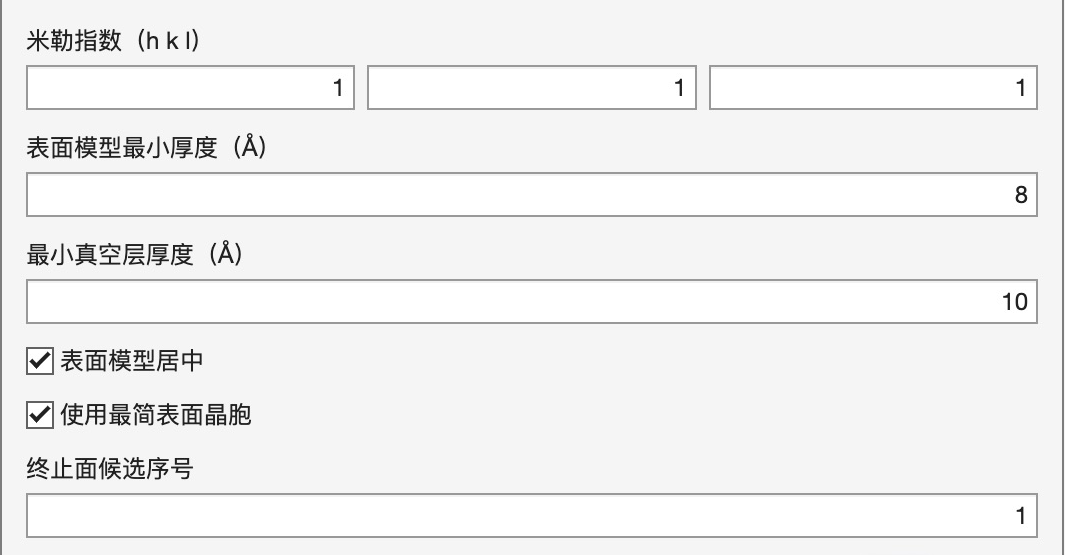
\includegraphics[width=107mm]{publication-assets/crop-e2fa9f70b6bcca245a04.png}
\par\vspace{2mm}
% 同图独立预览提示(975,1460,1520,1495)，545×35；54mm约256ppi，无右侧指针。

\includegraphics[width=54mm]{publication-assets/crop-f2ece60af591133fac37.png}
\caption{导入\file{Pt-fcc.cif}后构建Pt(111)表面的参数。米勒指数依次为1、1、1，最小表面厚度为$8\,\text{\AA}$，最小真空层厚度为$10\,\text{\AA}$；启用居中与最简表面晶胞，终止面候选序号为1。下方显示预览提示。}
\label{fig:pt111-slab-parameters}
\end{figure}


隨書\file{Pt-fcc.cif}與\file{Pt111-slab.cif}分別提供這一體相和表面模型。本組引數得到 4 個獨立位點、4 個幾何層。沿表面法向，晶胞週期高度約為 $20.3689\,\text{\AA}$，最外兩層原子平面的跨度約為 $6.7896\,\text{\AA}$，相鄰週期薄片的最外原子平面之間相隔約 $13.5793\,\text{\AA}$。構建厚度按晶體重複單元選取，與最外原子座標的差值不是同一種計量。測量時應沿表面法向投影；斜晶胞的第三條晶格向量長度不能直接當作真空厚度。

\subsection{固定底層原子}
\index{Guding yuanzi@固定原子}
\index{Zhenkong@真空層}

表面弛豫中常保留底部若干層，以近似較深處的體相約束。表面構建後，工具可以識別幾何層。開啟\ui{固定原子}，將底部幾何層數設為 1，可選擇最底部一層。若使用當前選擇而不是自動底層，應按介面設定將底層數置為 0，再明確選擇需要固定的位點。

固定標記儲存在模型中。提交計算時，在相應任務設定中啟用所需約束。對於較厚薄片，也可以固定多層；初次練習時先固定一層並檢視層的範圍，便於理解。

\subsection{留出真空層}

\ui{新增真空層}沿第三條晶格向量增加空間，輸入的是新增厚度。若該向量與表面法向傾斜，新增長度在法向的投影會小於輸入值；本例使用法向晶胞練習。例如再輸入 $5\,\text{\AA}$，表示在當前模型基礎上繼續增加空間，不是將總真空強制設為 $5\,\text{\AA}$。應用後從側面檢查晶胞與薄片的位置關係。吸附質或溶劑加入後，原先看起來充足的真空還可能被佔去一部分，因此應再次檢視完整模型。

新增真空的幾何關係為
\begin{equation}
  \mathbf c'=
  \frac{\|\mathbf c\|+\Delta}{\|\mathbf c\|}\,\mathbf c,
  \qquad
  \Delta H=\Delta\,
  \left|\frac{\mathbf c}{\|\mathbf c\|}\cdot\hat{\mathbf n}_{\mathrm{slab}}\right|.
  \label{eq:vacuum-addition-projection}
\end{equation}
$\Delta$和$\Delta H$的單位都是\AA。前者是輸入的新增長度，後者是法向胞高的增加量；點積給出的比例介於0和1之間。例如，第三晶格向量沿全域性$z$，表面法向沿$(1,1,1)$時，輸入$2\,\text{\AA}$只會增加約$2/\sqrt{3}=1.155\,\text{\AA}$的法向胞高。圖\ref{fig:surface-vacuum-geometry}中的$\Delta\mathbf c=\mathbf c'-\mathbf c$是長度為$\Delta$的增量，$\Delta H$是它的法向投影長度；將$\mathbf c$先整理到法向後，長度與實際間隔便容易對應。



\begin{steps}
  \item 重新匯入\file{Pt111-normal-c.json}，保留一份未修改的薄片。這份輸入的第三條晶格向量已沿表面法向。在\ui{晶體建模}的\ui{表面建模}中開啟\ui{新增真空層}。
  \item 新增厚度設為 $5\,\text{\AA}$。先預覽，從側面比較薄片與外框，確認改變的是薄片外的空間。
  \item 應用後再次核對 Pt 位點數和薄片內部幾何；增加真空不應增加 Pt 原子，也不應拉大薄片內部的層間距。
  \item 另存為\file{Pt111-extra-vacuum}，與原始薄片分別保留。後面的吸附練習仍從指定的原始檔案重新開始。
\end{steps}

\begin{figure}[H]
\centering
\begin{tikzpicture}[x=1mm,y=1mm,font=\sffamily\small,>=stealth]
  \foreach \shift in {0,65} {
    \fill[paleblue] (\shift+12,15) rectangle (\shift+44,25);
    \draw[teal] (\shift+12,15) -- (\shift+44,15);
    \draw[teal] (\shift+12,25) -- (\shift+44,25);
    \foreach \x in {16,25,34,43} {
      \fill[brand] (\shift+\x,18) circle (1.3);
      \fill[teal] (\shift+\x-2,22) circle (1.3);
    }
    \draw[->,brand,line width=.7pt] (\shift+12,6) -- (\shift+45,6)
      node[right] {$\mathbf a$};
    \draw[densely dashed,muted] (\shift+12,25) -- (\shift+12,53);
  }
  \node[text=brand] at (29,65) {倾斜的第三晶格矢量};
  \node[text=brand] at (94,65) {第三晶格矢量沿法向};
  \draw[->,brand,line width=.8pt] (12,6) -- (34,44)
    node[pos=.55,right] {$\mathbf c$};
  \draw[->,teal,line width=1pt] (34,44) -- (41,56)
    node[pos=.6,right] {$\Delta\mathbf c$};
  \draw[densely dashed,muted] (34,44) -- (51,44);
  \draw[densely dashed,muted] (41,56) -- (51,56);
  \draw[<->,teal] (49,44) -- (49,56);
  \node[anchor=south,text=teal,font=\sffamily\footnotesize] at (48,57) {$\Delta H$};
  \draw[->,muted,line width=.7pt] (6,28) -- (6,49)
    node[above] {$\hat{\mathbf n}$};
  \draw[->,brand,line width=.8pt] (77,6) -- (77,44)
    node[pos=.52,left] {$\mathbf c$};
  \draw[->,teal,line width=1pt] (77,44) -- (77,56)
    node[right] {$\Delta H=\Delta$};
  \node[align=center,font=\sffamily\footnotesize] at (29,-4)
    {法向增加量小于沿 $\mathbf c$ 的新增长度};
  \node[align=center,font=\sffamily\footnotesize] at (94,-4)
    {输入的新增长度就是法向增加量};
\end{tikzpicture}
\caption{添加真空层时的方向关系（截面示意）。薄片内部的相对位置保持不变，第三晶格矢量沿原方向伸长，工具同时将薄片重新居中；只有当它垂直于表面时，新增长度才全部用于增大法向间隔。}
\label{fig:surface-vacuum-geometry}
\end{figure}


\section{在表面放置吸附物}
\index{Xifu@吸附建模}

\subsection{確定吸附位置}

表面吸附建模需要回答三個問題：放在哪裡、以哪個原子連線、朝向哪邊。頂位（ontop）位於表面原子上方，橋位（bridge）位於兩個表面原子之間，空位（hollow）位於若干表面原子圍成的區域中。分子內部的錨定原子決定哪一個原子放在給定高度；取向原子則幫助確定分子的方向。

先用\ui{尋找吸附位點}觀察候選位置，可以把抽象的位點名稱與當前表面對應起來。預設高度為 $2\,\text{\AA}$。位點是生成初始構型的幾何參考，並不表示分子在該處已經達到穩定吸附。

\subsection{為吸附練習整理晶胞}

先重新匯入未經修改的\file{Pt111-slab.cif}。本節不使用前一節額外增加真空後的結構。這個表面的法向沿全域性座標的 $(1,1,1)$，原晶胞的 $c$ 向量卻沿全域性 $z$ 方向。當前引數命令沿 $c$ 方向增加錨點高度，因此先把 $c$ 調整到表面法向，可以使輸入高度與側檢視中的垂直距離一致。

開啟\ui{重定義晶胞}，保留 $a$、$b$ 兩行，只將 $c$ 行的 $x$、$y$、$z$ 三項分別設為 11.76、11.76、11.76，單位為 \AA；保持原子的笛卡爾位置。這裡採用的是 $c_{\mathrm{new}}=c+6a+6b$，沒有擴胞，仍有 4 個 Pt 位點。新的 $c$ 垂直於表面，面內 $a$ 與 $b$ 之間仍為 $60^\circ$。也可以直接匯入隨書的\file{Pt111-normal-c.json}，從已經整理好的晶胞開始。

從側面檢視薄片，再顯示晶胞邊框：$c$ 應沿表面向外，薄片內部的層間位置保持不變。對於其他表面，應根據其面內向量確認法向，不要直接套用本例的三項座標。

\subsection{示例：互動放置 \headinglatin{O--H} 片段}

互動方式適合觀察分子如何接近表面。它允許一邊拖動完整片段，一邊檢查高度、取向和接觸。

\begin{steps}
  \item 開啟已整理晶胞的 \file{Pt111-normal-c}，按 O 進入吸附物放置，選擇 O--H 片段。片段欄也可使用專案中的分子或使用者片段。
  \item 從表面原子向外拖動，建立表面位點與片段錨點之間的關係。調整檢視，使拖動方向容易判斷。
  \item 左鍵拖動改變整個片段的朝向；Alt+左鍵拖動調整錨定距離；右鍵拖動使片段繞錨定方向旋轉。
  \item 檢查 O--H 內部連線是否保持，片段是否與鄰近表面原子過近。預覽合適後按 Enter 或\ui{應用}提交。
  \item 儲存為獨立吸附模型。若要調整放置方式，可撤銷後重新操作。
\end{steps}

\subsection{示例：按引數向外放置 \headinglatin{O--H}}

引數方式便於記錄和重複相同的構型。隨書\file{oh-fragment.mol}含 O、H 兩個原子和一條單鍵，O--H 長度為 $0.96\,\text{\AA}$。先把它匯入專案，再重新匯入未經吸附修改的\file{Pt111-normal-c.json}並啟用新匯入的宿主，從乾淨的四位點薄片開始。

\begin{steps}
  \item 開啟\ui{放置吸附物}，在\ui{專案吸附物}下拉選單中選擇匯入的 O--H 分子。
  \item 位點型別選擇頂位（ontop），候選序號為 1，\ui{錨點高度（Å）}設為 2。
  \item 錨定原子設為 1，即 O；取向原子設為 2，即 H。在方向的三個數值框中分別填 1、1、1，使 O 指向 H 的方向與本例表面法向一致。最小允許距離保持 $0.5\,\text{\AA}$。
  \item 預覽後從側面檢查：O 應位於選定 Pt 原子的外側，H 在更遠的一端，再單擊\ui{應用}。
  \item 本例輸入含負的分數座標。為使宿主與吸附物在同一晶胞內檢視，開啟\ui{構建超胞}，三個縮放值都填1並應用。這一步把等價位點歸入單位晶胞，不擴大模型；晶格和6個獨立位點保持不變。
  \item 將結果改名為\file{Pt111-OH-outward}並儲存。開啟晶胞邊框，從側面檢查O--H朝向；邊界映像可能使同一片段顯示多次，應以摘要中的6個獨立位點核對組分。
\end{steps}

% Online实际参数放置与归胞后的侧视；只裁切原JPEG，不修改像素。
\begin{figure}[H]
\centering
% 3024×1758；(980,620,2045,1480)，1065×860；107mm约253ppi。
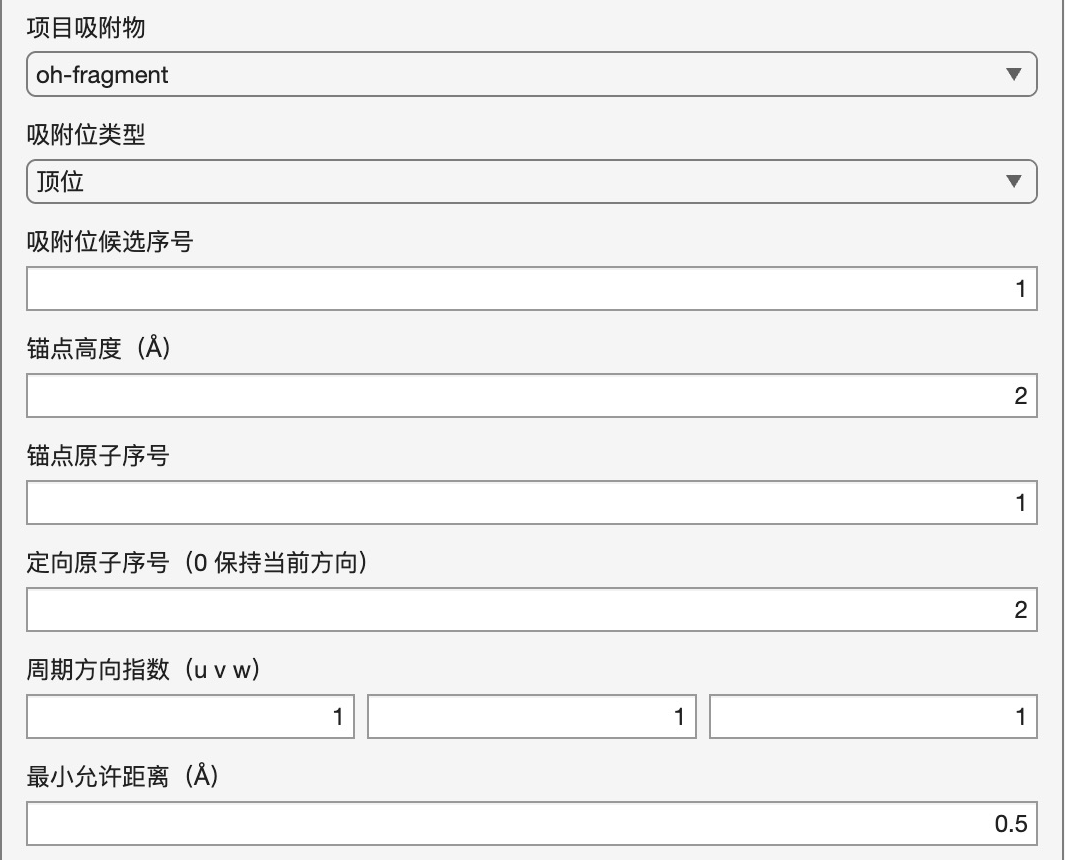
\includegraphics[width=107mm]{publication-assets/crop-c02e14aa8762e8947bbe.png}
\caption{向外放置O--H的参数。选择项目中的\file{oh-fragment}，顶位候选1，锚点高度$2\,\text{\AA}$，锚定原子1、定向原子2，周期方向指数依次为1、1、1，最小允许距离$0.5\,\text{\AA}$。本例先将宿主的$c$调整为表面法向。}
\label{fig:pt111-oh-parameters}
\end{figure}

\begin{figure}[H]
\centering
\begin{minipage}[t]{80mm}
\vspace{0pt}
% 完整晶胞(1000,360,2020,1685)，1020×1325；80mm约324ppi。
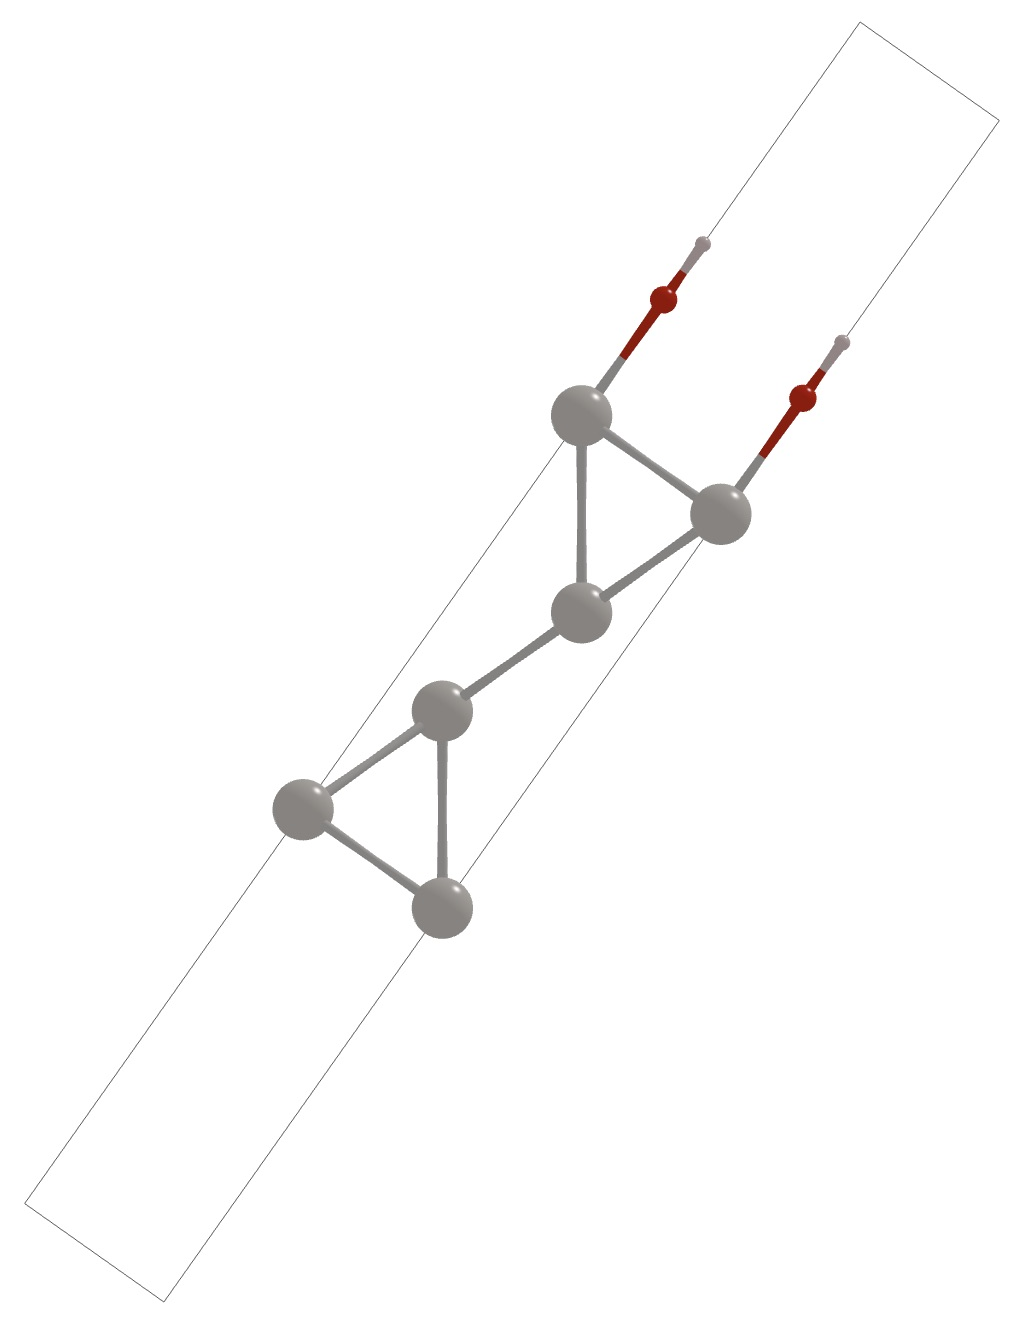
\includegraphics[width=\linewidth]{publication-assets/crop-c201c0495d5d847c2fd3.png}
\end{minipage}\hfill
\begin{minipage}[t]{40mm}
\vspace{0pt}
% 独立摘要(40,330,445,560)，405×230；40mm约257ppi。
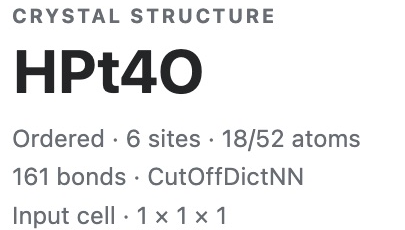
\includegraphics[width=\linewidth]{publication-assets/crop-5caa5064e4762ffc4974.png}
\end{minipage}
\caption{应用吸附放置并以$1\times1\times1$单位超胞归胞后的结构侧视。模型组成为$\mathrm{Pt_4OH}$，含6个独立位点；画面中的两个O--H为同一片段的周期映像。图中展示吸附物放置后的初始结构。}
\label{fig:pt111-oh-side}
\end{figure}


參考結果含 $\mathrm{Pt_4OH}$，共 6 個位點。O 距頂層平面 $2.00\,\text{\AA}$，H 距頂層平面 $2.96\,\text{\AA}$，O--H 長度保持 $0.96\,\text{\AA}$。隨書\file{Pt111-OH-outward.cif}可用來比較晶胞和原子位置；片段的顯式單鍵儲存在輸入 MOL 檔案中。若將取向原子改為 0，工具會保留片段原有朝向，因此相同錨點高度不一定得到同一取向。

隨書\file{Pt111-OH-Online-050.json}儲存歸胞後的六個位點，其週期幾何與上述結構相同，可直接用於檢視和繼續建模。吸附能需透過後續計算求得。

\subsection{批次比較吸附構型}

\ui{吸附構型定位器}可以列舉位點、高度和轉角，並按評分保留一組候選。先重新匯入未經吸附修改的\file{Pt111-normal-c.json}，啟用新匯入的四位點宿主，再選擇上述 O--H 分子。在\ui{位點型別}文字框中輸入 \literalinput{ontop bridge hollow}，在\ui{候選高度（Å）}文字框中輸入 \literalinput{1.8 2.1 2.4}，表示比較 $1.8$、$2.1$、$2.4\,\text{\AA}$ 三個高度。錨定原子設為 1，取向原子設為 0；旋轉步長設為 $30^\circ$，最小接觸距離 $0.6\,\text{\AA}$，最多保留 200 個候選，種子為 0。評分模型使用預設幾何接觸評分。

本組引數對應 144 個候選，各構型保持 O--H 長度，錨點位於指定的法向高度。\file{Pt111-OH-candidate-1.json}儲存幾何評分第一項：hollow 型別的候選 2，高度 $2.4\,\text{\AA}$，轉角 $60^\circ$。可以先將它與前面的頂位模型比較，再觀察其他候選的錨點和轉角。

這些值用於理解搜尋範圍。分子較大時，可先減少高度與轉角組合，確認錨點設定正確，再擴大搜尋。候選表中選定一項後，先\ui{預覽}，比較不同構型，再\ui{應用}所需候選。對後續需要分別弛豫的構型，應保留為多個清楚命名的模型。

預設幾何接觸評分反映構型的幾何適合程度；可選的 UFF 範德華相互作用能是在剛性模型下的相互作用估計。兩者適合篩選初始結構，不能替代弛豫後的吸附能。記錄研究結果時，同時說明構型來源與後續計算方法。

\section{處理表面邊界}

\subsection{鈍化未飽和表面}

\ui{表面鈍化}根據未飽和配位新增原子。引數包括鈍化元素、鍵長、處理上表面或下表面，以及表面探測深度。預設元素為 H、鍵長 $1.1\,\text{\AA}$、同時處理兩側、探測深度 $1.5\,\text{\AA}$。對於不同材料，應按目標化學結構選擇鍵長和配位數。目標配位設為 0 時由工具推斷；已知表面化學時可以明確指定。

\subsection{建立溶劑層}

\ui{新增溶劑層}把專案中的溶劑分子裝填到表面上方。應先準備並檢查單個溶劑分子，再設定分子數、層厚、表面間隔和剩餘真空。例如，20 個分子、層厚 $10\,\text{\AA}$、表面間隔 $2\,\text{\AA}$、剩餘真空 $5\,\text{\AA}$，構成一組容易檢視的練習輸入。接觸容差和隨機種子影響裝填結果；完成後從側面檢查分子層範圍，再從上方檢查區域性堆積。

\section{構建異質結}\label{sec:heterojunction}
\index{Cengpipei@層匹配}
\index{Yizhijie@異質結}

\subsection{理解兩種材料的共同晶胞}

異質結由兩種不同材料相接形成。對層狀介面，可以把兩側材料分別準備為薄片，再沿法向疊放。兩種材料原來的晶格通常不同；要把它們放入同一個週期計算模型，需要找到共同的面內晶胞，並決定允許多少形變。這個共同晶胞既描述介面的重複方式，也決定一次計算包含多少原子。

本節的\ui{堆疊異質結構}用於這類上下疊放的介面。它比較面內超胞與旋轉，隨後按指定間距組裝兩部分。石墨烯/h-BN 是便於觀察的小例子；從塊體材料建立薄膜介面時，先分別用\ui{構建表面模型}準備需要相接的晶面，檢查每一側的層數、終止面和組成，再進行匹配。材料名稱相同並不意味著表面取向已經相同，晶面選擇應先於介面組裝。

面內應變表示原有晶格為了共用一個週期而改變了多少，層間距表示兩部分初始分開的距離，面內平移則改變區域性原子如何上下對齊。三個量各有作用。建立幾何模型後，還可以在同一組計算條件下比較不同間距和堆垛；介面電荷轉移、能帶對齊等性質由後續電子結構計算分析。

\subsection{按位移插入結構}

\ui{插入結構}把專案中的另一結構放入當前模型，可指定笛卡爾平移向量和最小原子間距。它適合已經知道兩部分相對位置的情況。插入後應檢查晶胞、組成和跨邊界的鄰近接觸。

\subsection{尋找面內晶格匹配}

\ui{堆疊異質結構}進一步搜尋面內晶格匹配。需要選擇頂層結構，給定層間距、總真空、最大面內應變、重複範圍和旋轉範圍。預設層間距 $3.35\,\text{\AA}$ 只是介面初值，不能通用於所有材料。最大應變 0.03 表示 3\%，是無量綱約束；候選可以按應變、面積或原子數排序。

比較候選時，可以先看應變是否合理，再看晶胞面積與原子數能否滿足計算規模。最小應變候選不一定也是最小模型。選定候選後檢查兩層的面內方向、層間距離和真空，再為不同堆垛分別儲存結構。

\subsection{練習：比較直接插入與層匹配}

隨書\file{graphene-layer.json}是一個含兩個 C 位點的石墨烯層，面內晶格常數為 $2.46\,\text{\AA}$，盒高為 $15\,\text{\AA}$。面內週期重複，法向為非週期。先將它匯入兩次並分別命名為\file{bottom}和\file{top}，即可用同材雙層練習幾何操作。

直接插入時，啟用底層，開啟\ui{插入結構}，將專案中的另一結構設為頂層。在\ui{插入位移（笛卡爾，Å）}的三個數值框中，從左到右分別填 0、0、3.35，最小距離保持 $0.5\,\text{\AA}$。結果應有 4 個位點，兩層相隔 $3.35\,\text{\AA}$，原盒高仍為 $15\,\text{\AA}$。隨書\file{graphene-inserted.json}保留了這個狀態。

另從原始底層開始，開啟\ui{堆疊異質結構}，仍以\file{top}作為另一結構。層間距設為 $3.35\,\text{\AA}$，總真空為 $15\,\text{\AA}$，最大面內應變為 0.03，最大面內重複數為 2，最大旋轉搜尋角為 $0^\circ$，候選按面積排序。

在引數視窗將\ui{介面候選序號}設為1，預覽並應用，再檢視結果候選表。隨書參考結果列出10個候選，候選1的應變為0、預計4個位點。應用後得到盒高 $18.35\,\text{\AA}$、層間距 $3.35\,\text{\AA}$ 的雙層，對應\file{graphene-stacked.json}。比較兩種結果，可以看到直接插入保留原盒子，而層匹配構建按薄片與總真空重新安排法向尺寸。

候選列表還可能包含高於指定應變上限的組合；列出不表示可以直接應用。本例候選 2、3 的應變約為 52.49\%，應排除；候選 4、5、6 接近零應變，但需要 8 個位點。先檢查約束，再選擇面積或規模合適的候選，比只看排列影象更可靠。

\subsection{示例：石墨烯與 h-\headinglatin{BN} 的層匹配}

兩種材料的面內尺寸通常略有差別。本例將石墨烯與六方氮化硼（h-BN）疊放，觀察匹配時的應變。\file{hBN-layer.json}是含 B、N 各一個位點的理想單層，面內晶格常數為 $2.50\,\text{\AA}$；石墨烯的相應數值為 $2.46\,\text{\AA}$。兩份輸入的法向盒高均為 $15\,\text{\AA}$。

\begin{steps}
  \item 將\file{graphene-layer.json}與\file{hBN-layer.json}匯入同一專案。啟用新匯入的\file{graphene-layer}，開啟\ui{堆疊異質結構}，在\ui{上層結構}下拉選單中選擇\file{hBN-layer}。
  \item 層間距設為 $3.35\,\text{\AA}$，總真空設為 $15\,\text{\AA}$，最大面內應變設為 0.03。
  \item 最大面內重複數設為 1，最大旋轉搜尋角設為 $0^\circ$，候選按應變排序。先限制到這個小範圍，便於看清兩種晶格如何匹配。
  \item 在引數視窗將\ui{介面候選序號}設為1，預覽並應用，再從側面檢查層間距。應用後出現的候選表只有一項：面內應變為0.016，即1.6\%，預計4個位點。
\end{steps}

候選表用於檢視各組匹配，並不在表內提供切換構型的應用按鈕。比較其他候選時，先撤銷到原始底層，或重新匯入底層，再開啟同一命令並填寫需要的候選序號。不要在已經組裝的雙層上繼續疊加。

結果\file{graphene-hBN-stacked.json}含 $\mathrm{C_2BN}$，h-BN 的面內晶格匹配到石墨烯晶格；層間距為 $3.35\,\text{\AA}$，法向盒高為 $18.35\,\text{\AA}$。與同材雙層相比，本例需要有限的面內形變才能共用一個週期晶胞。後續可以擴大重複與旋轉範圍，比較更大的匹配晶胞，並分別儲存準備計算的構型。這裡的層間距是建模初值，弛豫後的距離需由相應計算確定。

\section{構建扭轉雙層}\label{sec:twisted-structures}
\index{Niuzhuan shuangceng@扭轉雙層}
\index{Moer chaojingge@莫爾超晶格}

\subsection{從相對轉角到共同週期}

將兩張石墨烯單層重疊，再使其中一層繞法向轉動，區域性的原子對齊關係就會隨位置改變：有些區域接近原子上下相對，有些區域接近一層原子落在另一層六元環中心。把視野擴大，可以看到這些區域性排列組成較大的重複圖案，稱為莫爾圖案。

用於週期計算的模型還需要一個共同晶胞。上層不能只在原來的小晶胞中任意旋轉，否則越過晶胞邊界後，兩層的排列通常接不上。\ui{扭轉莫爾超晶格}為兩層分別選擇整數超胞，使它們能夠放入同一面內週期。輸入的目標角用於尋找合適的匹配，最終模型則由一組具體的整數關係確定。

本節使用約 $21.7868^\circ$ 的石墨烯雙層作為第一例。這個轉角對應較小的共同週期，結果只有 28 個碳位點，便於同時觀察兩層和晶胞。先完成這個例子，再嘗試較小轉角，能夠更清楚地理解角度、週期和模型規模之間的關係。

\subsection{準備上下兩層}

本工具使用六方面內原胞：兩個面內晶格向量等長，夾角為 $60^\circ$ 或 $120^\circ$。本例的單層石墨烯包含兩個 C 位點，面內晶格常數為 $2.46\,\text{\AA}$，盒高為 $15\,\text{\AA}$。兩個面內方向週期重複，法向為非週期。

隨書的\file{twist-graphene-bottom.json}與\file{twist-graphene-top.json}來自同一份單層輸入，分別供底層和上層使用。它們與前面\file{graphene-layer.json}的幾何相同。兩份檔案分開命名，是為了讓專案中的角色一目瞭然，不表示兩層已具有不同轉角。

\begin{steps}
  \item 把兩份 JSON 匯入同一專案，分別將結構命名為\file{twist-bottom}和\file{twist-top}。
  \item 開啟底層的三維文件，檢查它只有兩個模型位點。螢幕上用於顯示週期連線的映像原子可以多於兩個。
  \item 檢視晶格，確認面內長度均為 $2.46\,\text{\AA}$、夾角約為 $120^\circ$。再檢查上層具有相同的晶格和組成。
  \item 啟用\file{twist-bottom}。在頂部\ui{晶體建模}的\ui{表面與介面}區域開啟\ui{介面建模}，選擇\ui{扭轉莫爾超晶格}。
  \item 在\ui{上層結構}下拉選單中選擇\file{twist-top}。這裡選的是專案中已有的結構，不是在輸入框中填寫磁碟路徑。
\end{steps}

第一次練習應從這兩張原始單層開始。前面已經插入或堆疊過的雙層可另行保留，不能再把它當成一張原始單層送入本例。

\subsection{填寫一組小規模引數}

\begin{table}[htbp]
\centering
\caption{28位點石墨烯扭轉雙層的練習引數。}
\begin{tabularx}{\linewidth}{lX}
\toprule
引數 & 本例輸入與含義\\
\midrule
上層結構 & 在下拉選單中選擇\file{twist-top}。\\
角度（度） & 輸入\literalinput{21.786789}，作為目標相對轉角。\\
層間距（Å） & 輸入 3.35，規定兩張單層之間的初始間隔。\\
總真空層厚度（Å） & 輸入 15，規定薄片之外的總空白高度。\\
允許的最大面內應變 & 輸入 0.03，即 3\%。\\
最大原子數 & 輸入 200，限制生成模型的總位點規模。\\
最大週期匹配指數 & 輸入 6，限定整數匹配的搜尋範圍。\\
\bottomrule
\end{tabularx}
\end{table}

\ui{角度（度）}是一個數值框，輸入的是度數；不需要再寫度符號。\ui{層間距}和\ui{總真空層厚度}也都是長度數值。最大應變則是比例，0.03 表示 3\%，不能把 3 直接填作同一個要求。

最大原子數不是要求軟體一定生成 200 個原子，而是允許的上限。最大週期匹配指數也不是沿某個方向簡單重複 6 次。工具會在這個範圍內尋找整數匹配，綜合考慮目標角偏差、應變和結構大小，再選出一組結果。因此，這兩個上限與\ui{構建超胞}中的三個重複倍數有不同含義。

本命令內部選擇一組匹配，不提供\ui{堆疊異質結構}那樣的候選排序和候選序號欄位。填寫完引數後，應檢查生成結構的實際規模和相對取向；需要比較其他匹配時，保留原始兩層，分別生成和儲存各組引數的結果。

\begin{steps}
  \item 按表填寫引數，先使用\ui{預覽}檢查。模型應從兩個位點的單層變成兩層組成的較大週期結構。
  \item 沿接近表面法向觀察，檢查兩層的六元環排列已經相對轉動；轉到側面，確認仍然只有兩層，層間沒有意外插入其他原子。
  \item 檢查模型位點總數應為 28。面內晶胞擴大後，檢視器的顯示映像數仍可能多於這個數。
  \item 應用後把結果命名為\file{graphene-twist-21p786789}，儲存專案。保留兩份輸入單層，使後續比較可以從同一起點開始。
\end{steps}

\begin{figure}[H]
\centering
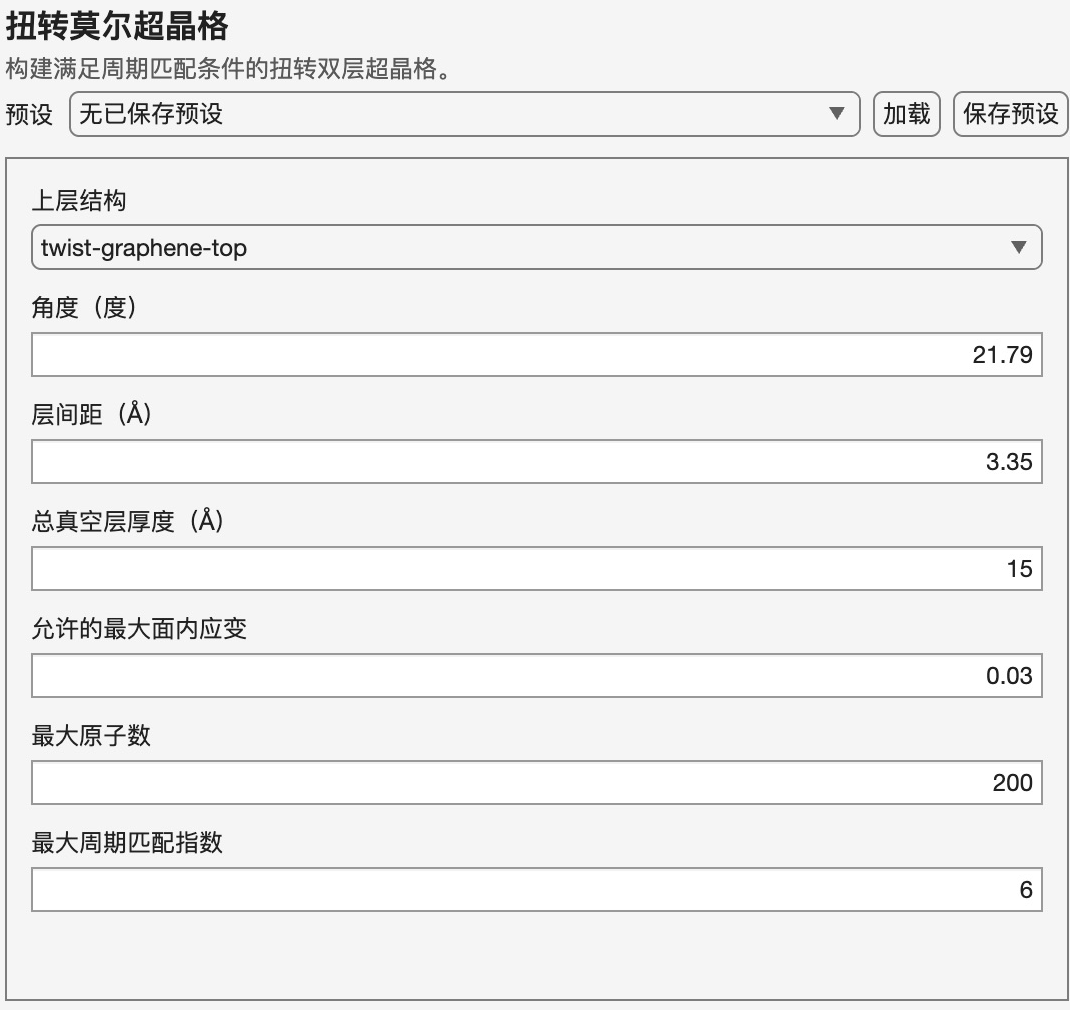
\includegraphics[width=107mm]{publication-assets/crop-7c221ceb9a35fdad53a3.png}
\par\vspace{2mm}

\includegraphics[width=60mm]{publication-assets/crop-faecdf5879e359505e34.png}
\caption{扭轉引數與預覽結果。目標角輸入21.786789度；數值框失去焦點後按顯示精度呈現為21.79。上層在圖中保留匯入時的名稱\file{twist-graphene-top}，對應本節的\file{twist-top}；預覽生成28個位點。}
\label{fig:online-twist-parameters}
\end{figure}

\begin{figure}[H]
\centering
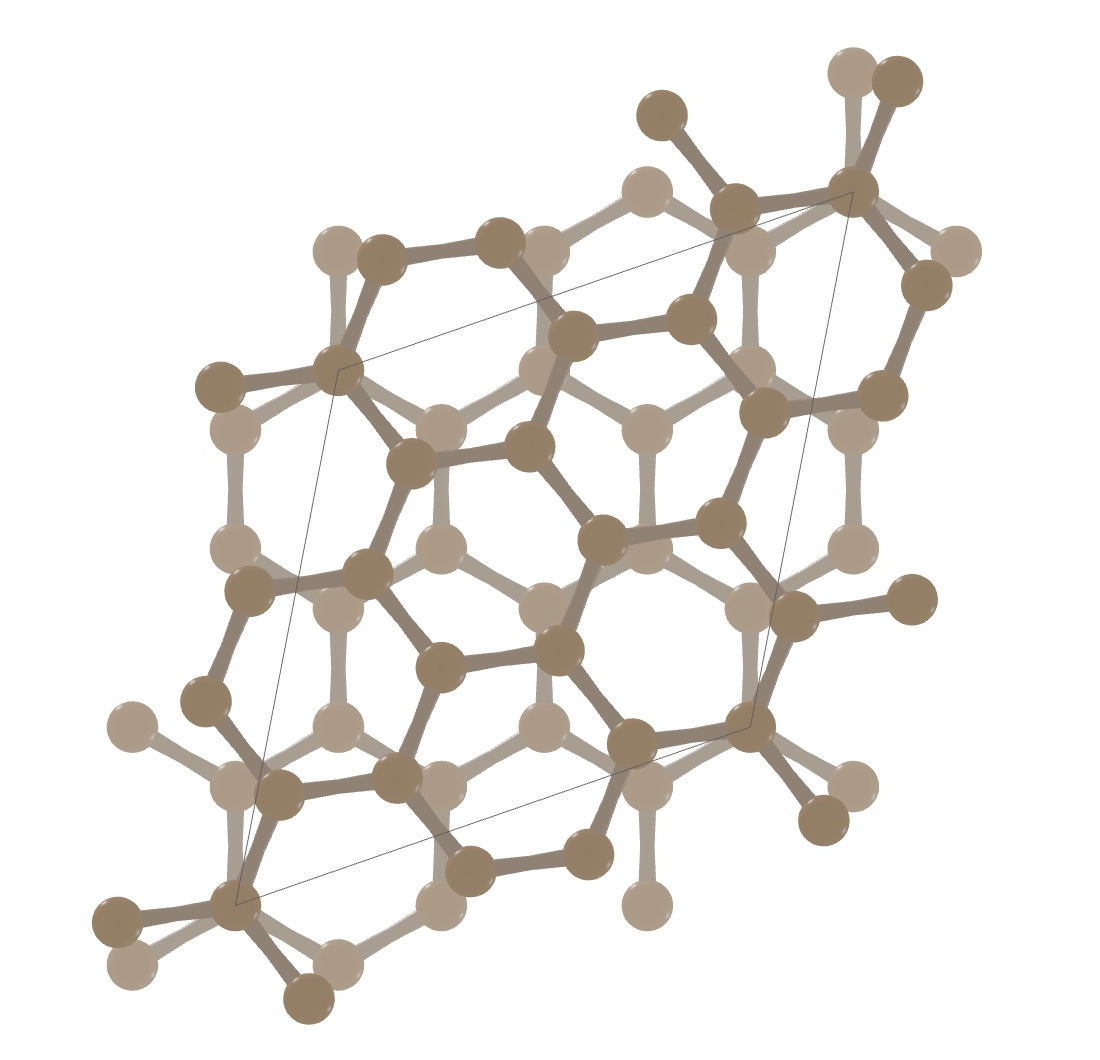
\includegraphics[width=93mm]{publication-assets/crop-89eb072a4598add87b05.png}
\caption{石墨烯扭轉雙層的法向檢視。兩層的六元環相對轉動；28個模型位點按當前週期範圍顯示為68個原子。}
\label{fig:online-twist-top}
\end{figure}

\subsection{讀懂生成的晶胞}

隨書\file{graphene-twist-21p786789.json}是按上述引數得到的參考結構，另提供幾何交換用的同名 CIF。模型有 28 個 C 位點，分為兩層，每層 14 個。與原始每層兩個位點相比，每一層的面內面積擴大為原來的 7 倍。

面內兩個晶格向量等長，均約為 $6.508548\,\text{\AA}$。相應面積約為 $36.6859\,\text{\AA}^2$。本例的新面內夾角為 $60^\circ$；輸入原胞的夾角為 $120^\circ$，兩者是不同的晶格基底表示，不能只憑角度改變就判斷晶體被拉歪。核對長度、面積、位點數與兩層的週期連線，應當放在一起進行。

對於這組石墨烯輸入，週期邊長也可用 $\sqrt{7}\times2.46\,\text{\AA}$ 核對，約為 $0.651\,\mathrm{nm}$。這裡的週期描述共同晶胞在面內的重複長度，不是層間距離，也不是某條 C--C 鍵長。模型中每層最短近鄰距離仍約為 $1.420282\,\text{\AA}$，與輸入單層一致。

從側面看，兩層相隔 $3.35\,\text{\AA}$，法向胞高為 $18.35\,\text{\AA}$。這組模型中每層原子各在一個平面內，所以本例胞高等於層間距與總真空之和。總真空 $15\,\text{\AA}$ 是整個薄片之外的空白高度；它不表示薄片上方和下方各有 $15\,\text{\AA}$。

\begin{figure}[H]
\centering
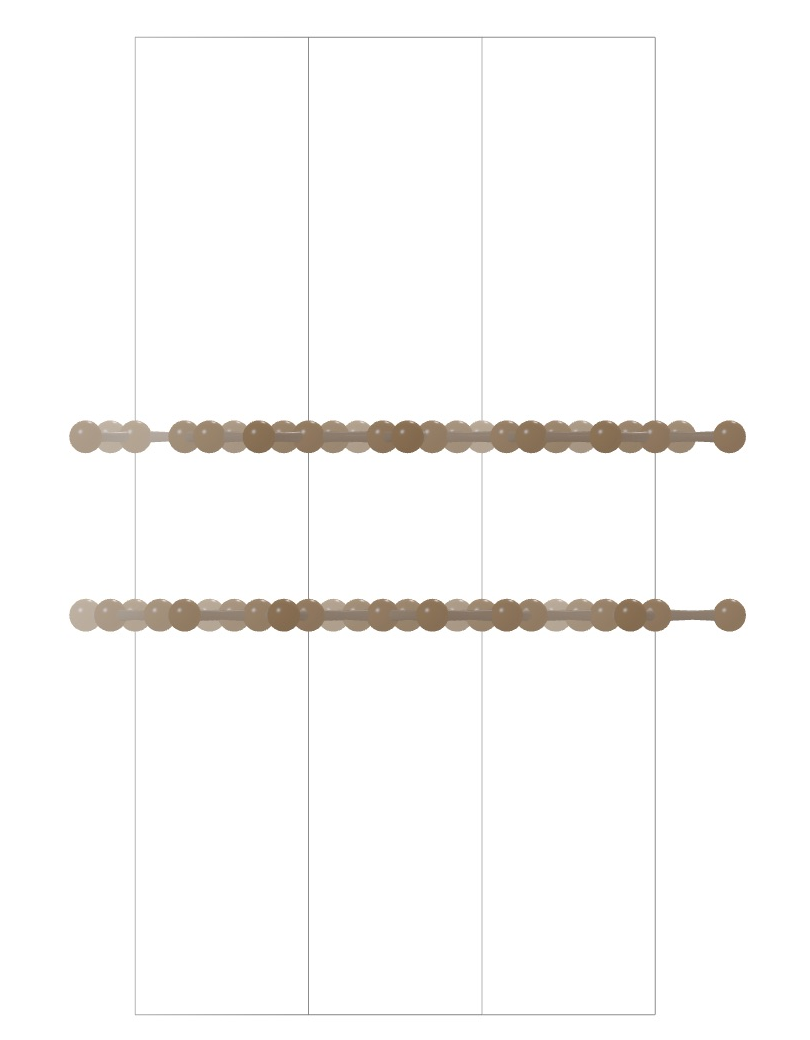
\includegraphics[width=67mm]{publication-assets/crop-a8d161a93e2745b16ef3.png}
\caption{同一模型的側視。兩張原子平面與法向晶胞邊界一起顯示，便於分辨層間距離和外側真空。}
\label{fig:online-twist-side}
\end{figure}

隨書參考結構的實際匹配角為 $21.786789298^\circ$，與目標角相差約 $2.98\times10^{-7}$ 度，面內應變為 0。檢查兩層近鄰鍵的方向，也可得到這一相對角度。

精確的角度和匹配資訊儲存在原生 JSON 的\file{properties}下的\file{moire}部分。用普通文字編輯器開啟本例 JSON，搜尋\file{achieved_angle_degrees}即可找到實際角；\file{target_angle_degrees}是目標角，\file{angle_error_degrees}是兩者的偏差，\file{in_plane_strain}是面內應變。對自己生成的結構，在檢視器的\ui{Export file}中選擇\ui{Structure file}，再選 JSON 匯出。不應選擇同一選單裡的\ui{Scene JSON}，後者儲存檢視場景，不能用來查詢上述結構匹配資訊。

\subsection{目標角與實際角為什麼可能不同}

目標角的輸入範圍為 $0^\circ$ 到 $60^\circ$。按六方面內晶格的對稱關係，工具把實際匹配角表示在 $0^\circ$ 到 $30^\circ$ 之間；比較較大目標角時，也應按這一表示約定檢視結果。本節先在這個較小範圍內練習，便於直接比較目標值與實際值。

共同週期只能由特定整數關係構成。輸入一個任意小數角，並不意味著一定存在大小合適、又完全等於該角的週期胞。本例把目標改成 $22^\circ$，保持其他引數不變，仍然得到 28 位點結構，實際角仍約為 $21.786789298^\circ$，角度偏差約為 $0.213211^\circ$。

這兩次構建具有相同的最終幾何，卻對應不同的目標輸入。隨書\file{graphene-twist-target22.json}保留了第二次結果，便於比較。報告模型時，應記錄實際角，而不是隻把引數視窗中輸入的目標角寫進圖題。

\begin{table}[htbp]
\centering
\caption{本組輸入下目標角與規模限制的實際對照。}
\begin{tabularx}{\linewidth}{lX}
\toprule
輸入變化 & 實際生成結果\\
\midrule
目標 $21.786789^\circ$，上限200 & 28位點，實際約 $21.786789298^\circ$。\\
目標 $22^\circ$，上限200 & 仍為28位點和同一實際角，偏差約 $0.213211^\circ$。\\
目標 $21.786789^\circ$，上限24 & 本例選擇4位點、接近 $0^\circ$ 的匹配，未達到原目標。\\
\bottomrule
\end{tabularx}
\end{table}

第三行說明，完成構建與達到目標角是兩項不同的檢查。28位點的匹配被上限24排除後，工具會在剩餘範圍內選擇結果。構建後，看到數量與預期明顯不同，應回到引數和實際角一起核對，再決定是否增大搜尋範圍。

較小轉角通常需要較長的共同週期和更多原子。比較不同轉角時，可以先固定層間距與應變要求，再逐步增加允許的模型規模和匹配指數。這樣更容易看清新增的搜尋範圍究竟改善了角度匹配，還是隻帶來更大的結構。本節約 $21.8^\circ$ 的例子使用較小整數，適合作為操作和週期檢查的起點。

\subsection{按研究目的選擇組裝入口}

\ui{介面建模}選單把幾種組裝方式放在一起。選擇時，先明確已經知道哪些幾何關係，再決定讓工具尋找什麼。

\begin{table}[htbp]
\centering
\caption{直接插入、層匹配與扭轉構建的選擇。}
\begin{tabularx}{\linewidth}{lX}
\toprule
入口 & 適合開始的情形\\
\midrule
插入結構 & 兩部分的位置已經確定，只需給出相對平移；保留當前宿主晶胞。\\
堆疊異質結構 & 希望比較共同面內晶胞，從允許應變、重複範圍與旋轉範圍中選擇候選。\\
扭轉莫爾超晶格 & 已有六方單層和目標轉角，希望尋找相應的整數共同週期。\\
\bottomrule
\end{tabularx}
\end{table}

在\ui{堆疊異質結構}的候選表中，面積、應變、原子數和旋轉角各自回答不同問題。面積與原子數反映計算規模；應變說明原始晶格需要改變多少才能匹配；旋轉角說明兩層如何相對定向。應變很小的候選也可能很大，面積最小的候選也可能需要較大形變。先比較這些量，再看具體原子排列，選擇會更有依據。

本節的扭轉命令則先利用六方整數關係確定一組共同週期，再組裝兩層。它不會要求在同一個視窗中填寫\ui{候選序號}。如果希望比較目標 $21.786789^\circ$ 與 $22^\circ$，應分別從兩張原始單層構建，分別記錄結果，而不是在前一個已完成的雙層上再次施加相同命令。

同樣，直接旋轉螢幕上的觀察方向只會改變視角；選擇一組原子進行旋轉則改變原子位置。兩者都不能代替共同晶胞的週期匹配。檢查扭轉模型時，除觀察兩層取向，還應顯示晶胞邊框，沿兩個面內方向檢視重複後的連線，確認區域性圖案與整個週期表達的是同一模型。

這組入口用於沿法向疊放的層狀介面。構建面內並排相接的異質結時，需另行準備結區的原子排列與邊界。

\subsection{進一步建立石墨烯/h-\headinglatin{BN}扭轉異質結構}

扭轉不只用於同一種材料的雙層。前面石墨烯與 h-BN 的零轉角匹配，主要展示兩種面內晶格常數如何協調；在此基礎上，還可以同時引入相對轉角。本例仍使用石墨烯作為底層，h-BN 作為上層：石墨烯晶格常數為 $2.46\,\text{\AA}$，h-BN 為 $2.50\,\text{\AA}$。

\begin{steps}
  \item 重新匯入\file{twist-graphene-bottom.json}與\file{hBN-layer.json}，分別命名為\file{graphene-bottom}和\file{hBN-top}。不要把前一個已經扭轉的雙層作為底層。
  \item 啟用新的石墨烯單層，在\ui{扭轉莫爾超晶格}中將\ui{上層結構}選擇為\file{hBN-top}。
  \item 沿用表中的目標角、層間距、總真空、200位點上限與匹配指數6，允許最大面內應變仍設為0.03。
  \item 預覽後核對組成應為 $\mathrm{C_{14}B_7N_7}$，共28個位點。上層和底層各有14個位點，但元素組成不同。
  \item 應用並儲存為\file{graphene-hBN-twist-21p786789}，再與零轉角的\file{graphene-hBN-stacked.json}比較。
\end{steps}

本例實際角同樣約為 $21.786789298^\circ$，面內主應變為 0.016，即 1.6\%。h-BN 的面內尺寸被匹配到石墨烯共同晶格，層間距仍為 $3.35\,\text{\AA}$，法向胞高仍為 $18.35\,\text{\AA}$。應變和轉角描述的是不同變化：前者調整尺寸，後者改變兩層的相對方向。

兩種構建命令得到的都是幾何模型。研究介面電荷轉移、能帶對齊或結區性質時，需要在儲存的結構上繼續建立相應計算，並區分構建輸入的層間距與計算後得到的距離。

\subsection{儲存扭轉模型}

儲存專案可以保留輸入層、生成結構和後續工作流。單獨交換結構時，本組提供 JSON 與 CIF 兩種格式：JSON保留面內/法向週期標記、層編號和扭轉匹配資訊；CIF便於交換晶胞與原子位置。匯入本組CIF時，三個方向均按週期處理，莫爾匹配資訊需另行保留。繼續本章的二維建模比較，優先使用JSON；使用CIF進入其他計算流程時，再按目標方法確認法向邊界與真空設定。

\begin{steps}
  \item 為每個結果寫清材料、實際角和主要變化，例如“石墨烯雙層，實際21.7868度”，不要只儲存\file{result}之類的通用名稱。
  \item 記錄輸入層的晶格、目標角與實際角、應變、層間距、總真空、位點數及面內週期。比較表可將這些量各佔一列。
  \item 儲存專案後重新開啟，再檢查上下兩層的組成和晶胞。匯出結構時，保留對應的引數記錄，便於解釋另一個軟體中看到的模型。
  \item 需要重複生成時，以\file{-nojvm}啟動MATLAB\regmark{}，配置好工具箱路徑後，從隨書示例目錄執行\file{twist_examples.m}；只檢查已儲存檔案時，執行\file{verify_twist_examples.m}。
\end{steps}

隨書結構是用於後續弛豫和電子結構計算的初始模型。比較扭角效應時，採用一致的泛函、贗勢、截斷能和合適的取樣條件，並將計算設定與結構一同儲存。


\section{準備 \headinglatin{NEB} 初始路徑}

\ui{生成 NEB 路徑}需要專案中的初態與終態。兩端結構必須具有相同的原子數量、元素排列與晶格，才能使原子一一對應。預設生成 5 箇中間構型，並用 IDPP 改善插值中的原子間距。生成後逐幅檢查移動軌跡和近距離接觸；這些中間結構用於後續路徑計算，反應能壘由能量計算確定。

\subsubsection{中間構型怎樣分佈}

若填寫$M$箇中間構型，連同兩端共有$M+2$個結構。以$j=0,\ldots,M+1$編號。對於非週期模型，或已選定連續週期映像的兩端，線性插值的位置關係為
\begin{equation}
  \alpha_j=\frac{j}{M+1},\qquad
  \mathbf r_i^{(j)}=(1-\alpha_j)\mathbf r_i^{(0)}
     +\alpha_j\mathbf r_i^{(M+1)}.
  \label{eq:neb-image-interpolation}
\end{equation}
$i$表示同一個原子在兩端對應的序號，$\alpha_j$是無量綱路徑引數，位置以\AA 表示。週期結構還要按所用週期邊界處理端點位移，不能將同一原子在兩個不同週期映像中的座標直接當作很長的遷移距離。

IDPP進一步使每個構型中的原子對距離接近插值目標：
\begin{equation}
\begin{aligned}
  d_{ik}^{*,(j)}&=(1-\alpha_j)d_{ik}^{(0)}
                      +\alpha_j d_{ik}^{(M+1)},\\
  E_{\mathrm{IDPP}}^{(j)}&=
    \sum_{i<k}\frac{\bigl(d_{ik}^{(j)}-d_{ik}^{*,(j)}\bigr)^2}
                         {\bigl(d_{ik}^{(j)}\bigr)^4}.
\end{aligned}
\label{eq:idpp-pair-objective}
\end{equation}
其中$i,k$為原子序號，$j$為構型序號；$d_{ik}^{(j)}$是當前原子對距離，$d_{ik}^{*,(j)}$是對應的目標距離。分母使過短的原子間距受到較強懲罰，因此IDPP往往能改善線性插值中的碰撞。上式給出單個構型的原子對目標；路徑最佳化還會考慮相鄰構型之間的聯絡。

$E_{\mathrm{IDPP}}$是幾何插值的輔助目標，其值用於評價路徑幾何；反應能壘需由後續能量計算確定。視窗中的\ui{IDPP力收斂閾值}用於這一步輔助最佳化，與電子結構計算中的原子力閾值分別設定。$M=5$時，路徑引數依次為$0,1/6,2/6,\ldots,1$；本例的00至06正好對應七個結構。


\subsection{練習：檢查五個中間構型}
\index{NEB@NEB 路徑}

隨書\file{neb-exchange/initial.json}與\file{final.json}提供一個容易看清原子對應的幾何例子。兩個帶有不同標籤的 H 原子在 $10\,\text{\AA}$ 的非週期立方盒中交換位置：初態座標為 $(2,5,5)$ 和 $(8,5,5)\,\text{\AA}$，終態將這兩個位置對調。這裡研究的是插值如何避開原子重合，不把它作為氫分子反應。

\begin{steps}
  \item 把兩份端點檔案匯入同一專案，分別命名為\file{initial}與\file{final}。核對兩端原子順序與標籤一致，再啟用初態。
  \item 在\ui{晶體建模}的\ui{表面與介面}區域，開啟\ui{介面建模}，選擇\ui{生成 NEB 路徑}。在\ui{NEB 終態結構}下拉選單中選擇專案內的終態\literalinput{final}。
  \item \ui{NEB 中間構型數}設為 5，\ui{IDPP 最大最佳化步數}保持 200，\ui{IDPP 力收斂閾值}保持 0.1。預覽並應用後，在專案瀏覽器的結構分組中找到\literalinput{NEB image 00}至\literalinput{NEB image 06}，依次開啟。這7個結構包含兩端和5箇中間構型。
  \item 依序觀察原子標籤和兩點距離。兩端應保持原座標，中間構型則繞開原來會重合的位置。儲存當前專案，即可同時保留兩端輸入和這7個結果；需要單獨交換某幅時，再匯出相應結構。
\end{steps}

若直接作直線插值，兩個原子會在中間一幅重合。參考路徑的 IDPP 最佳化經 82 次迭代達到閾值，全路徑最短的兩點距離約為 $3.5755\,\text{\AA}$，中間一幅約為 $3.7380\,\text{\AA}$。\file{image-00.json}至\file{image-06.json}儲存全部路徑結構，便於逐幅比較。IDPP 報告中的目標值和數值力用於評價初始路徑，不是後續電子結構計算的能量和原子力。

圖~\ref{fig:neb-idpp}~把這些座標與直線插值放在一起比較。左圖中的線段連線已生成的結構，右圖給出相應兩點距離；沿圖號檢查，可以同時確認兩端不變和中間接觸改善。

\begin{figure}[H]
\centering
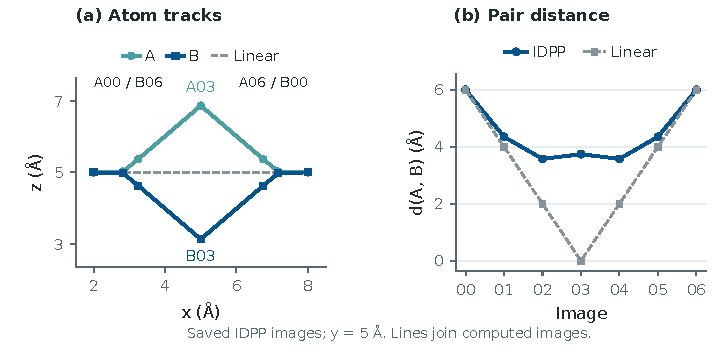
\includegraphics[width=\linewidth]{publication-assets/vector-79e6f35b7afec0271551.pdf}
\caption{兩個原子交換位置的 IDPP 參考路徑。左：固定 $y=5\,\text{\AA}$ 時的 $x$--$z$ 軌跡，A00/B06 等標籤標出端點對應；右：00至06各構型的兩點距離。灰色虛線為直線插值，03為中間構型。}
\label{fig:neb-idpp}
\end{figure}

\section{示例：建立低維模型}\label{sec:nanostructure-examples}
\index{Namidai@奈米帶}\index{Namiguan@奈米管}\index{Namixian@奈米線}

把片層裁成帶，或沿一個方向捲成管，會改變結構的邊界和週期。奈米帶在寬度方向出現邊緣，只沿長度方向重複；奈米管沿軸向重複，另外兩個方向留出真空。由塊體擷取的奈米線也只有一個週期方向；有限團簇則在三個方向都不重複。

本節先用一份小的石墨烯原胞建立24位點奈米帶和32位點奈米管，再從面心立方銅建立奈米線、有限團簇和球形空洞。每個結果都配有原生JSON與CIF檔案，可一邊構建，一邊與隨書結果比較。

\subsection{準備六十度石墨烯原胞}

隨書\file{nano-graphene-60.json}含兩個C位點，面內兩個晶格向量長度均為 $2.46\,\text{\AA}$，夾角 $60^\circ$，法向盒高 $15\,\text{\AA}$；兩個面內方向週期，法向非週期。它與前面的\file{graphene-layer.json}表示同一張石墨烯，區別是晶格基底的選取。

若從前面的 $120^\circ$ 原胞出發，可保留 $\mathbf a$，將第二個向量換成 $\mathbf a+\mathbf b$。新向量仍長 $2.46\,\text{\AA}$，但與 $\mathbf a$ 的夾角成為 $60^\circ$。這次整數換基的行列式為1，因此不會擴大模型，仍有兩個獨立位點。本節的帶和管均使用這份 $60^\circ$ 輸入。

\begin{steps}
  \item 將\file{nano-graphene-60.json}匯入專案，命名為\file{nano-graphene}，開啟三維文件，檢查兩個獨立位點、等長的面內晶格和 $60^\circ$ 夾角。
  \item 如希望自己換基，另行匯入原始\file{graphene-layer.json}並啟用。在\ui{晶體建模}\,$\rightarrow$\,\ui{超胞與晶格}中開啟\ui{構建超胞}。
  \item 在\ui{超胞倍率或變換矩陣}文字框中輸入\literalinput{1 0 0; 1 1 0; 0 0 1}。這是三行整數矩陣，分號用於分行；與編輯晶格視窗的逐格表格不同。
  \item 預覽後核對位點數仍為2，晶胞體積保持不變，面內夾角變為 $60^\circ$。應用後另存為能說明基底的名稱，不覆蓋原來的 $120^\circ$ 單層。
  \item 為奈米帶與奈米管分別保留一份輸入。每次構建都從單層開始，不能在已經裁成帶的結果上繼續執行卷管而當作同一個例子。
\end{steps}

兩種基底的晶胞邊框看起來不同，但原材料的週期幾何相同。使用本節命令時，先核對輸入檔案與基底，再比較位點數和尺寸；只抄寫寬度或手性指數，不足以確定同一個構建過程。

\subsection{裁出一條扶手椅邊石墨烯奈米帶}

奈米帶的寬度和軸向長度按重複單元數填寫；真空以\AA 為單位。\ui{armchair}與\ui{zigzag}描述兩種不同的邊緣排列，不是兩個相機方向。這裡選擇扶手椅邊，先檢查邊緣上的碳原子怎樣成對排列，再看沿帶長方向的週期連線。

\begin{table}[htbp]
\centering\small
\caption{24位點扶手椅邊奈米帶的引數。}
\begin{tabularx}{\linewidth}{lX}
\toprule
欄位 & 本例輸入\\
\midrule
寬度方向重複單元數 & 3，無量綱整數。\\
軸向重複單元數 & 2，無量綱整數。\\
邊緣型別 & 選擇\ui{armchair}。\\
真空層厚度（Å） & 5；本工具在兩個非週期方向的兩側分別留出該空白。\\
最大原子數 & 500；是構建規模上限，不是要求最終有500個位點。\\
\bottomrule
\end{tabularx}
\end{table}

\begin{steps}
  \item 啟用準備好的\file{nano-graphene}單層。從\ui{晶體建模}的\ui{奈米結構}選單開啟\ui{擷取奈米帶}。
  \item 按表填寫引數。寬度3不是 $3\,\text{\AA}$；軸向2也不是 $2\,\text{\AA}$。
  \item 單擊\ui{預覽}，顯示晶胞邊框。沿片層法向檢視兩條邊，轉到側面確認模型仍是一張平帶。
  \item 檢查獨立位點數為24，所有原子均為C。沿週期方向檢視接續，不能把靠近晶胞兩端的同一週期網路看成兩段斷開的分子。
  \item 應用後命名為\file{graphene-armchair-w3-l2}，儲存專案，並與隨書同名JSON比較。原單層仍需單獨保留。
\end{steps}

本例輸出在全域性 $y$ 方向週期，原生週期標記為\literalinput{false true false}。三個胞長約為 $16.15$、$8.521690$、$10.00\,\text{\AA}$。其中沿帶長的週期為 $8.521690\,\text{\AA}$；原子在寬度方向的實際跨度為 $6.15\,\text{\AA}$，再加兩側各 $5\,\text{\AA}$ 空白，得到 $16.15\,\text{\AA}$ 的盒寬。平片本身沒有法向厚度，所以該方向的盒長為 $10\,\text{\AA}$。

未鈍化的24個C原子中，以 $1.65\,\text{\AA}$ 為近鄰檢查界限，有16個原子連線三個近鄰，8個邊緣原子連線兩個近鄰；最短週期原子間距約為 $1.420282\,\text{\AA}$。這個界限用於核對這組碳模型，並不是所有元素的通用成鍵距離。若要研究氫鈍化邊緣，應另存未鈍化模型，再按目標邊緣配位新增氫並檢查組成。

\subsection{把石墨烯捲成一根小奈米管}

捲曲前先確定平面中哪一條向量將成為管的圓周。幫助資訊中的幾何關係為
\begin{equation}
  \mathbf C_h=n\mathbf a_1+m\mathbf a_2,
  \qquad R=\frac{\|\mathbf C_h\|}{2\pi}.
  \label{eq:nanotube-circumference-radius}
\end{equation}
$\mathbf a_1,\mathbf a_2$是輸入片層的面內晶格向量，單位為\AA；$n,m$是無量綱手性指數，$\mathbf C_h$是手性向量，$R$為初始管半徑。圓周長度取兩個基矢線性組合的模。等長、夾角$60^\circ$的面內基矢給出$\|\mathbf C_h\|=a\sqrt{n^2+nm+m^2}$；換用其他基底時，應回到式\eqref{eq:nanotube-circumference-radius}計算。本節沿用已整理好的$60^\circ$輸入；不同基底中的同一組$(n,m)$不應直接視為同一捲曲方向。

\begin{figure}[htbp]
\centering
\begin{tikzpicture}[x=1mm,y=1mm,font=\sffamily\small,>=stealth]
  \node[text=brand] at (26,54) {平面中的卷曲方向};
  \foreach \j in {0,1,2,3} {
    \draw[teal!55] ({6+4*\j},{10+7*\j}) -- ({38+4*\j},{10+7*\j});
    \foreach \i in {0,1,2,3,4} {
      \fill[brand] ({6+8*\i+4*\j},{10+7*\j}) circle (.8);
    }
  }
  \foreach \i in {0,1,2,3,4}
    \draw[teal!55] ({6+8*\i},10) -- ({18+8*\i},31);
  \draw[->,brand,line width=.9pt] (6,10) -- (38,10)
    node[midway,below=3pt] {$\mathbf C_h=4\mathbf a_1$};
  \draw[->,muted] (6,10) -- (14,10) node[above] {$\mathbf a_1$};
  \draw[->,muted] (6,10) -- (10,17) node[left] {$\mathbf a_2$};
  \draw[->,teal,line width=.8pt] (57,24) -- (69,24);
  \node[text=muted,font=\sffamily\footnotesize] at (63,32) {卷合};
  \node[text=brand] at (95,54) {圆周长度不变};
  \fill[paleblue] (81,10) rectangle (109,39);
  \draw[brand,line width=.8pt] (81,10) -- (81,39);
  \draw[brand,line width=.8pt] (109,10) -- (109,39);
  \draw[brand,fill=paleblue,line width=.8pt] (95,39) ellipse (14 and 5);
  \draw[brand,line width=.8pt] (81,10) arc[start angle=180,end angle=360,x radius=14mm,y radius=5mm];
  \draw[brand,densely dashed] (109,10) arc[start angle=0,end angle=180,x radius=14mm,y radius=5mm];
  \draw[->,muted] (95,39) -- (109,39) node[midway,above] {$R$};
  \draw[->,teal] (115,10) -- (115,43) node[above] {管轴};
  \node[align=center,font=\sffamily\footnotesize] at (95,-1) {$\|\mathbf C_h\|=2\pi R$};
\end{tikzpicture}
\caption{手性矢量与管半径的关系（示意）。左图的点表示晶格平移点，以$(4,0)$标出卷成一周的平面方向；右图表示卷曲后圆周与半径的几何关系。}
\label{fig:nanotube-chiral-geometry}
\end{figure}


手性指數 $(n,m)$ 指定捲成圓周的晶格方向，軸向重複數決定沿管軸保留多少個平移週期。本例使用 $(4,0)$，管半徑較小，便於觀察捲曲、接縫與週期。穩定半徑需在幾何弛豫後確定。

\begin{steps}
  \item 回到原始\file{nano-graphene-60.json}，另開一份單層文件並啟用。不要使用剛生成的奈米帶。
  \item 在\ui{奈米結構}選單選擇\ui{生成奈米管}。在\ui{手性指數（n m）}的兩個數值框中分別填4與0。
  \item \ui{軸向重複單元數}設為2，\ui{真空層厚度（Å）}設為6，\ui{最大原子數}設為500。
  \item 預覽後沿管軸觀察環形截面，再從側面檢查管身。轉動相機檢視卷合位置，並核對軸向兩端能按週期相接。
  \item 檢查模型共有32個C位點。應用後儲存為\file{graphene-tube-4-0-l2}，保留單層輸入和奈米管結果。
\end{steps}

本例沿全域性 $z$ 方向週期，週期標記為\literalinput{false false true}。由捲曲圓周得到的半徑為
\[
 R=\frac{4\times2.46}{2\pi}\,\text{\AA}\approx1.566085\,\text{\AA}.
\]
兩個橫向胞長均約為 $15.132169\,\text{\AA}$，等於管直徑加兩側各 $6\,\text{\AA}$ 真空；軸向胞長約為 $8.521690\,\text{\AA}$。本工具的橫向真空與扭轉雙層視窗中的\ui{總真空層厚度}含義不同，比較盒長時應按各命令的定義計算。

對儲存座標作週期近鄰檢查，32個位點均有三個距離小於 $1.65\,\text{\AA}$ 的近鄰，最短間距約為 $1.393202\,\text{\AA}$。平片捲成很小的圓周後，兩點之間的直線距離會與平面上的距離不同。因此，不必要求卷管後的全部C--C直線距離仍恰好等於平片的 $1.420282\,\text{\AA}$；應同時檢查半徑、接縫、近鄰與週期，後續幾何弛豫另行進行。

\subsection{從管口與側面閱讀奈米管}

已構建的奈米管也可以直接從隨書\file{graphene-tube-4-0-l2.json}匯入。這樣可以先熟悉觀察方法，再回到引數視窗比較不同的手性指數。初次取景保持\ui{Input cell}與\ui{1 × 1 × 1}，使畫面對應儲存的一個模型週期。

\begin{steps}
  \item 在\ui{主頁 → 結構 → 從檔案匯入結構}中選擇該JSON；線上版先上傳，再從雲檔案匯入。開啟結構文件，確認元素為C，模型摘要為32個位點。
  \item 在檢視工具欄單擊\ui{c}，其提示為\ui{View along c axis}。本例管軸與$c$平行，因此現在從管口看向管內；觀察碳原子圍成的環和中央空心區域。
  \item 單擊\ui{a}或\ui{b}轉到側面。保持相同縮放，檢查管身沿軸向延伸，六元環在曲面上的排列仍可辨認。若球體遮住連線，在\ui{Viewer settings → Style}中適度減小\ui{Atom scale}，再檢視區域性。
  \item 在\ui{Visibility}中顯示\ui{Unit cell}，把細長的管身與橫向真空盒比較。需要看清單個週期的原子時，可先隱藏\ui{Boundary image atoms}；檢查兩端接續時再顯示邊界映像。
  \item 在\ui{Scientific scene → Repeat cell}中只把\ui{c}設為2，觀察軸向兩段怎樣接上。看完使用\ui{Reset to 1 × 1 × 1}恢復，最後單擊\ui{Reset camera}重新取全景。
  \item 分別匯出管口和側面圖片，記錄兩圖來自同一32位點結構，並註明$(4,0)$、軸向兩個重複單元及原始JSON檔名。
\end{steps}

沿管軸看見“孔”，說明當前座標圍成了管形；側面和重複顯示則幫助確認它沿軸向週期延伸。顯示重複沒有把輸入改成更大的計算超胞。邊界附近增加的球體也屬於場景映像，模型獨立位點數仍應按原始結構讀取。以這兩種取向共同說明形態，比只留一張斜檢視更容易辨認管徑、管長與週期。

\begin{figure}[!htb]
\centering
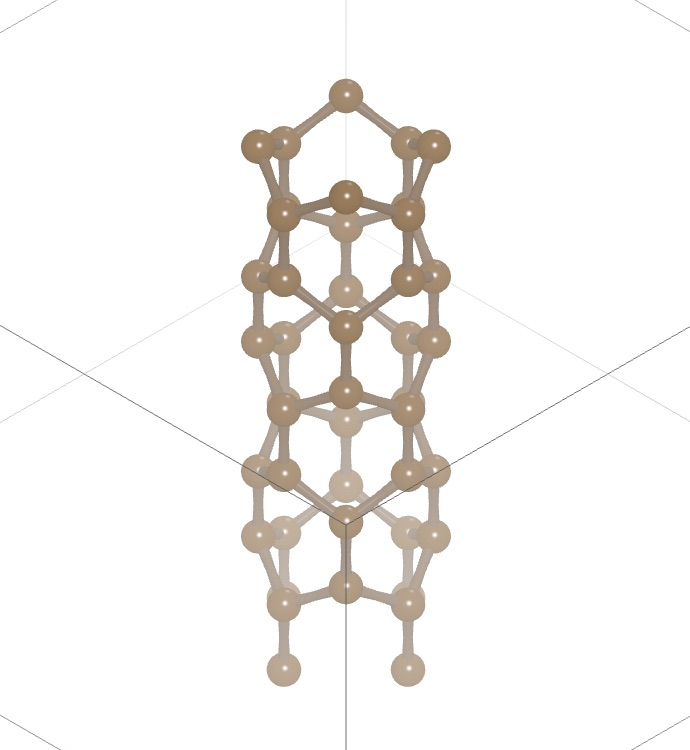
\includegraphics[width=.47\linewidth]{publication-assets/revision-nanotube-perspective.png}\hfill
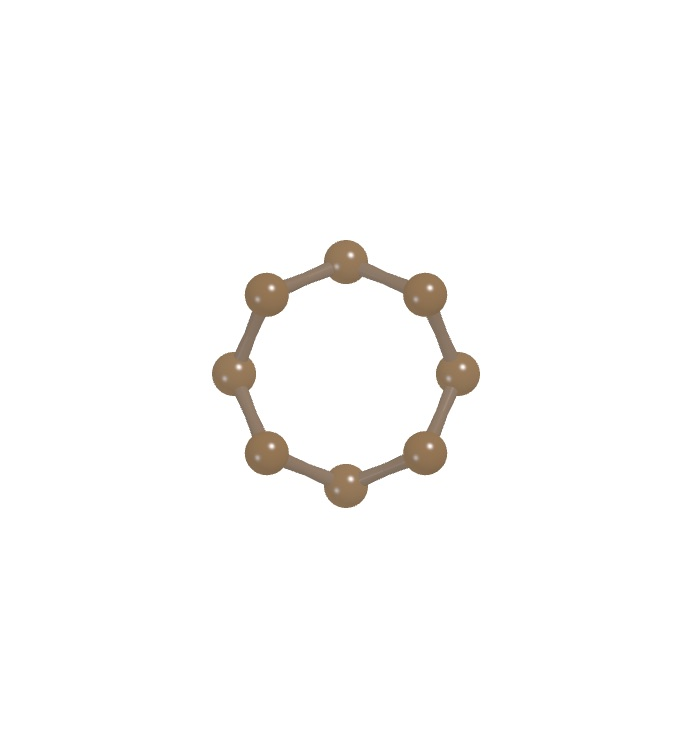
\includegraphics[width=.47\linewidth]{publication-assets/revision-nanotube-axis-c.png}
\caption{同一32位點碳奈米管的三維檢視。左：從側面檢查曲面的碳網路和軸向連線；右：沿管口方向觀察中央空心區域。顯示中包含週期邊界映像，獨立位點數保持32。}
\label{fig:nanotube-live}
\end{figure}

\FloatBarrier
\subsection{從銅晶體擷取奈米線}

銅例子使用隨書\file{nano-Cu-fcc-input.json}，與\file{Cu-fcc.cif}來自相同的四位點面心立方晶胞，晶格常數為 $3.61\,\text{\AA}$。奈米線保留一個晶格方向的平移週期，橫截面則按給定半徑擷取。擷取球或圓柱時，原子不是連續分佈的介質；實際最外原子的跨度不一定等於兩倍輸入半徑。

週期方向指數$[u\,v\,w]$透過實空間晶格給出線軸方向：
\begin{equation}
  \mathbf t=u\mathbf a+v\mathbf b+w\mathbf c.
  \label{eq:nanowire-lattice-direction}
\end{equation}
$u,v,w$為無量綱整數，$\mathbf t$與晶格向量使用相同的長度單位。構建時取與$\mathbf t$平行的軸，再以給定半徑保留橫截面內的原子；軸向週期長度以輸出晶胞為準。

\begin{table}[htbp]
\centering
\caption{晶格方向指標與晶面指標的區別。}
\begin{tabularx}{\linewidth}{lX}
\toprule
輸入 & 對應的幾何關係與用途\\
\midrule
$[u\,v\,w]$方向 & 由實空間的$\mathbf a,\mathbf b,\mathbf c$組合得到，用於奈米線軸向等方向選擇。\\
$(hkl)$晶面 & 由倒格矢組合得到法向，見式\eqref{eq:surface-miller-normal}，用於表面切割。\\
\bottomrule
\end{tabularx}
\end{table}

在立方晶胞中，同一組三個整數給出的方向與同指數晶面的法向平行；在一般斜晶胞中並非如此。填寫前先看視窗要求的是方向還是晶面，再從軸向和側向檢查預覽。

\begin{steps}
  \item 匯入銅輸入並啟用，在\ui{奈米結構}中開啟\ui{擷取奈米線}。
  \item 在\ui{週期方向指數（u v w）}的三個框中分別填0、0、1；半徑設為 $3\,\text{\AA}$，軸向重複單元數設為2，真空層厚度設為 $4\,\text{\AA}$，最大原子數設為2000。
  \item 預覽時沿線軸觀察截面，確認原子位於選定圓柱內。再從側面看軸向接續，核對共有24個Cu位點。
  \item 應用並儲存為\file{Cu-wire-001-r3-l2}。改變半徑或方向時，從原始銅晶體重新開始，避免把有限橫截面再次當成塊體擷取。
\end{steps}

結果沿 $z$ 軸週期，週期標記為\literalinput{false false true}，軸向胞長為 $7.22\,\text{\AA}$。兩個橫向原子跨度均為 $5.415\,\text{\AA}$，加上兩側各 $4\,\text{\AA}$ 的空白後，兩個橫向盒長均為 $13.415\,\text{\AA}$。最短週期近鄰距離約 $2.552655\,\text{\AA}$，與輸入面心立方銅的最近鄰距離相同。

最大原子數同時約束構建時需要的母超胞規模。本例採用2000；若上限過小，按提示檢查母超胞的規模後再調整。

\begin{figure}[!htb]
\centering
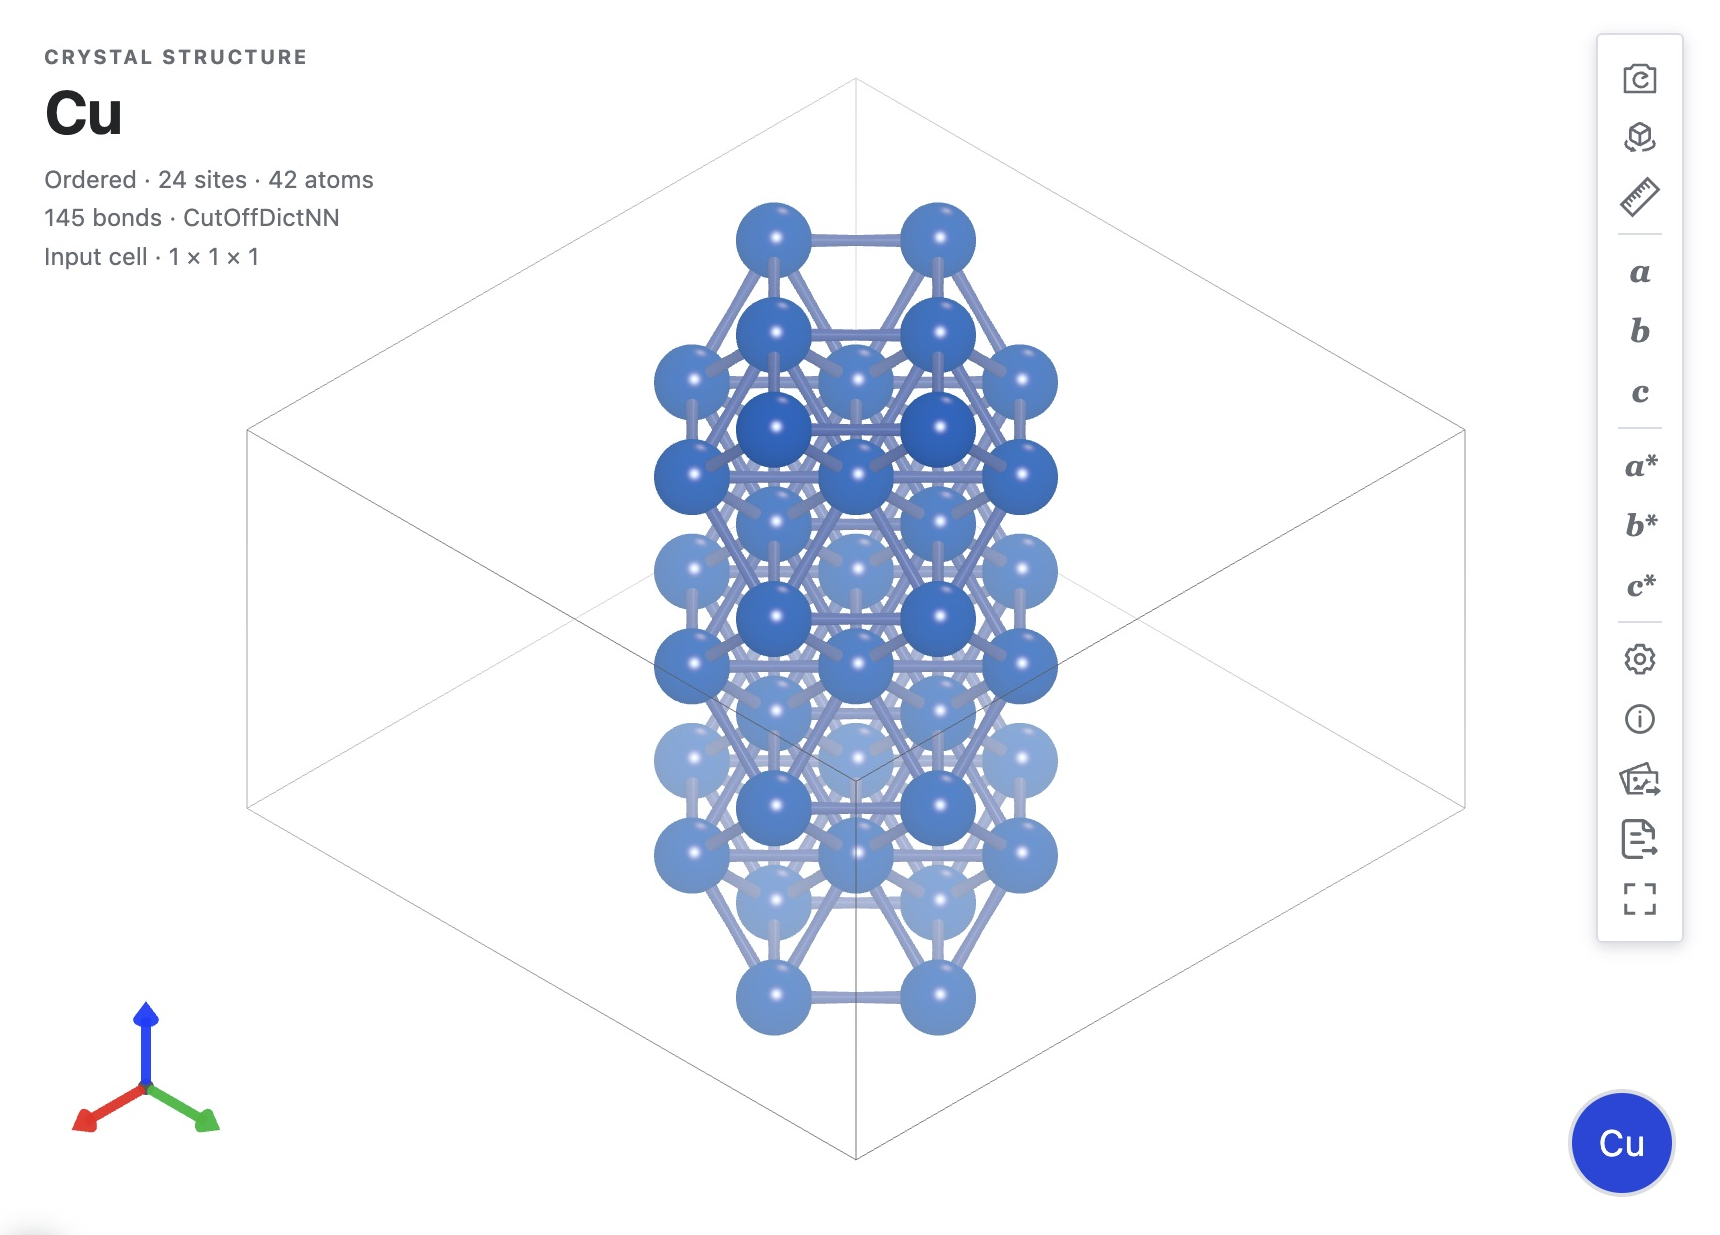
\includegraphics[width=\linewidth]{publication-assets/revision-nanowire-perspective.png}
\caption{隨書24位點銅奈米線的實際顯示。檢視器補出週期邊界原子以展示軸向連線，橫向的空白屬於真空區域。}
\label{fig:nanowire-live}
\end{figure}

\FloatBarrier
\subsection{檢查奈米線的截面與軸向}

開啟隨書\file{Cu-wire-001-r3-l2.json}，即可檢查已經擷取的24位點銅奈米線。它與奈米管都沿$c$方向週期。奈米管由單層捲成空心圓周；銅奈米線保留圓柱範圍內的晶體原子，橫截面內部也有原子。

\begin{steps}
  \item 匯入JSON並開啟三維文件，保持\ui{Input cell}。核對元素為Cu、獨立位點為24。
  \item 單擊檢視工具欄的\ui{c}沿線軸觀察截面。原子排列在離散的晶格位置上，輪廓可以呈階梯狀，不必形成光滑圓邊。
  \item 單擊\ui{a}或\ui{b}看側面，開啟\ui{Unit cell}。用軸向$7.22\,\text{\AA}$與橫向$13.415\,\text{\AA}$的盒長解釋取景：沿軸向是重複週期，橫向大盒用於容納有限截面與真空。
  \item 清除無關選擇，稍微旋轉為同時看見截面和側面的斜檢視。保留晶胞邊框與方位標記，檢查沒有原子被檢視邊緣裁掉。
  \item 按需要將\ui{Repeat cell}的\ui{c}設為2檢視接續，隨後恢復一個週期。儲存專案與結構；匯出圖片時在圖註記錄$[001]$方向、輸入擷取半徑$3\,\text{\AA}$和24個位點。
\end{steps}

輸入半徑決定保留哪些晶格位置，圖中最外原子的跨度則由實際保留的離散位置決定。本例橫向跨度$5.415\,\text{\AA}$小於直徑$6\,\text{\AA}$，與擷取規則一致。後續結構最佳化及電子性質分析可使用相應計算工作流。

\subsection{擷取一個有限銅團簇}
\index{Liangzidian@量子點}

\ui{量子點 / 奈米空洞}的\ui{量子點}模式保留球內原子，建立三個方向均不周期的有限結構。本例用13位點銅團簇觀察有限邊界與週期塊體的區別，儲存後可繼續安排相應的電子結構計算。

\begin{steps}
  \item 重新啟用四位點銅輸入，從\ui{奈米結構}開啟\ui{量子點 / 奈米空洞}。
  \item 處理方式選擇\ui{量子點}，半徑填 $3\,\text{\AA}$，真空層厚度填 $4\,\text{\AA}$，最大原子數設為2000。
  \item 預覽後旋轉觀察，確認沒有一條方向繼續連線成無限原子鏈。檢查共有13個Cu位點。
  \item 應用並命名為\file{Cu-dot-r3}，儲存專案和結構。
\end{steps}

本例的三個胞長均約為 $11.61\,\text{\AA}$，原子在各方向的跨度均為 $3.61\,\text{\AA}$，三向週期標記均為false。最短原子間距約 $2.552655\,\text{\AA}$。按 $2.8\,\text{\AA}$ 的近鄰界限檢查，中心原子有12個近鄰，其餘12個表面原子各有5個近鄰。這一初始團簇從面心立方排列直接裁取，穩定構型需進一步最佳化。

\subsection{在週期銅中挖出球形空洞}
\index{Namikongdong@奈米空洞}

空洞模式保留球外宿主和原週期盒；它與保留球內原子的量子點模式正好相反。先建立足夠大的宿主，可以避免只從很小晶胞中刪去大部分甚至全部原子。

\begin{steps}
  \item 匯入隨書\file{Cu-void-host-2x2x2.json}，或從四位點銅輸入透過\ui{構建超胞}建立 $2\times2\times2$ 宿主。應有32個Cu位點，三個胞長均為 $7.22\,\text{\AA}$。
  \item 啟用這份宿主，開啟\ui{量子點 / 奈米空洞}，處理方式選擇\ui{奈米空洞}，半徑設為 $2.7\,\text{\AA}$。空洞模式不需要為有限團簇增加外部真空。
  \item 預覽並顯示晶胞邊框。空洞中心固定在宿主的分數座標 \((0.5,0.5,0.5)\)，應檢查晶胞中央的原子被移除，而外圍週期宿主仍保留。
  \item 核對本例移除13個原子，剩餘19個Cu位點；晶格仍為 $7.22\,\text{\AA}$ 的立方胞，三個方向繼續週期。
  \item 應用後另存為\file{Cu-void-r2p7}，保留完整32位點宿主，便於以後改變半徑或比較缺陷。
\end{steps}

剩餘原子距空洞中心的最短週期距離為 $3.61\,\text{\AA}$。這個值大於輸入半徑 $2.7\,\text{\AA}$，反映了晶格上可保留的位置是離散的，不表示半徑欄位失效。剩餘宿主的最短原子間距仍約 $2.552655\,\text{\AA}$。儲存時同時記錄“輸入刪除球半徑”和“剩餘最近原子距中心”，會比只給一張透檢視更清楚。

\subsection{檢查週期並儲存配套檔案}

每個例子的原生JSON保留當前晶格、座標、週期標記及相應構建資訊；CIF用於交換晶胞和原子幾何。匯入本組CIF時，三個方向均按週期處理。繼續低維建模並保留本節的週期方向時，應使用JSON。

\begin{table}[htbp]
\centering\small
\caption{隨書奈米結構的位點數與原生週期。}
\begin{tabularx}{\linewidth}{lX}
\toprule
結果 & 實際模型與主要檢查值\\
\midrule
石墨烯奈米帶 & 24C；僅$y$週期；軸向 $8.521690\,\text{\AA}$。\\
$(4,0)$奈米管 & 32C；僅$z$週期；半徑 $1.566085\,\text{\AA}$。\\
銅奈米線 & 24Cu；僅$z$週期；軸向 $7.22\,\text{\AA}$。\\
銅團簇 & 13Cu；三個方向非週期；盒長各 $11.61\,\text{\AA}$。\\
帶空洞的銅 & 19Cu；三個方向週期；32位點宿主中移除13個。\\
\bottomrule
\end{tabularx}
\end{table}

\begin{steps}
  \item 先儲存專案，確認輸入結構和派生結果具有不同名稱。
  \item 如需單獨結構檔案，在檢視器的\ui{Export file}\,$\rightarrow$\,\ui{Structure file}中選JSON，保留模型資訊；幾何交換可另存CIF。這裡不要選擇用於顯示場景的\ui{Scene JSON}。
  \item 重新開啟儲存的結構，檢查位點數、晶胞和週期方向；再檢查邊緣、卷合處或球形裁切邊界的近鄰。
  \item 需要重新生成這組結構時，以\file{-nojvm}啟動MATLAB\regmark{}，配置好工具箱路徑後，從隨書示例目錄執行\file{nano_examples.m}。\file{verify_nano_examples.m}用於檢查已有結構。
\end{steps}

本節提供未鈍化的初始模型，可根據材料與邊界需要繼續鈍化、弛豫和電子結構計算。將模型接入工作流時，儲存構建引數與計算引數，並確認工作流引用所需的結構。


\section{示例：建立高分子鏈}
\index{Gaofenzi@高分子}

\subsection{理解重複單元}

高分子建模從重複單元開始。PE、PP、PS、PEO、PPO 等內建單元可以直接呼叫；使用者重複單元則需要明確頭原子、尾原子和連線時移去的原子。頭尾定義決定相鄰單元如何連線，因此儲存重複單元前，應先檢查單體拓撲。

均聚物只使用一種重複單元，嵌段共聚物把不同單元組成連續段，無規共聚物則按組成和隨機規則生成序列。鏈序列與空間構象是兩類引數：相同的 PE/PP 序列，可以採用伸展、折線或無規線團初始構象。種子用於重現相同的隨機構建條件。

\subsection{\headinglatin{PEO--PPO--PEO} 嵌段}

\begin{steps}
  \item 啟用分子文件，在頂部\ui{分子建模}的\ui{軟物質}區域開啟\ui{聚合物建模}，選擇\ui{構建嵌段共聚物}。
  \item 在\ui{嵌段重複單元}文字框中輸入 \literalinput{PEO PPO PEO}，在\ui{嵌段長度}文字框中輸入 \literalinput{3 4 3}，均用空格分隔各項。完整嵌段超單元重複次數設為 1，鏈數設為 1。
  \item 種子設為 8，\ui{初始構象}下拉選單先選擇\ui{伸展}，首尾端基文字框保持 \file{none}。
  \item 檢視預計原子數，預覽並應用。檢查總共有 10 個重複單元，其中 PEO 合計 6 個，PPO 為 4 個。
  \item 從整體觀察鏈序列，再放大檢視兩個嵌段交界處的連線。儲存為能夠表達序列的名稱，例如 \file{PEO3-PPO4-PEO3}。
\end{steps}

隨書\file{PEO3-PPO4-PEO3.json}由上述引數生成，組成為 $\mathrm{C_{24}H_{50}O_{10}}$，共 84 個原子、83 條鍵。10 個重複單元連成一條鏈，相鄰單元之間有 9 條連線。雖然端基輸入為\file{none}，鏈兩端尚未滿足的價鍵仍由氫補足；核對分子式時應把這些氫計入。

% 插入第8章PEO3–PPO4–PEO3组成段后；本片段不自动修改第8章。
% 全部引用Online原生截图，以独立LaTeX矩形裁切排版，不修改像素。
\begin{figure}[H]
\centering
% 100%浏览器图的核心参数(980,580,2040,1030)，1060×450；105mm约256ppi。
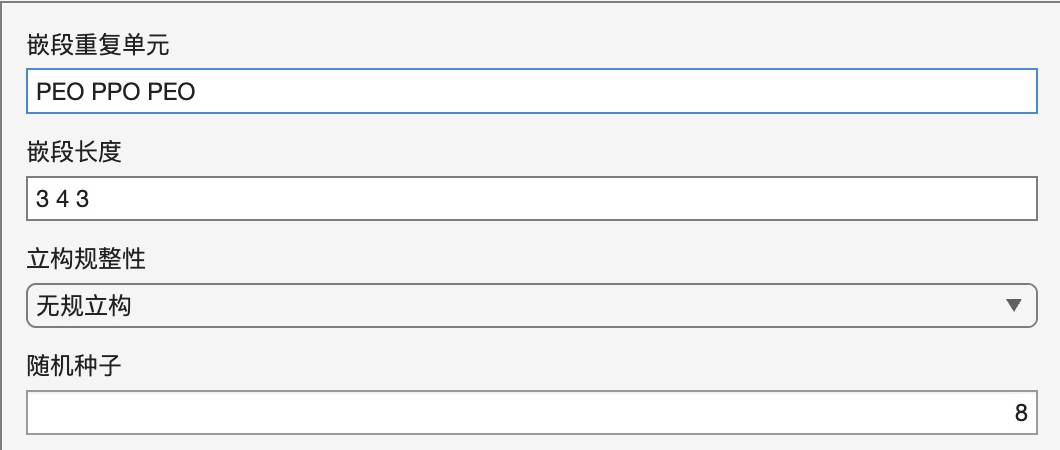
\includegraphics[width=105mm]{publication-assets/crop-3d7aab6f859860340b2f.png}
\par\vspace{3mm}
% 125%浏览器图中下部完整字段(845,710,2175,1535)，1330×825；122mm约277ppi。
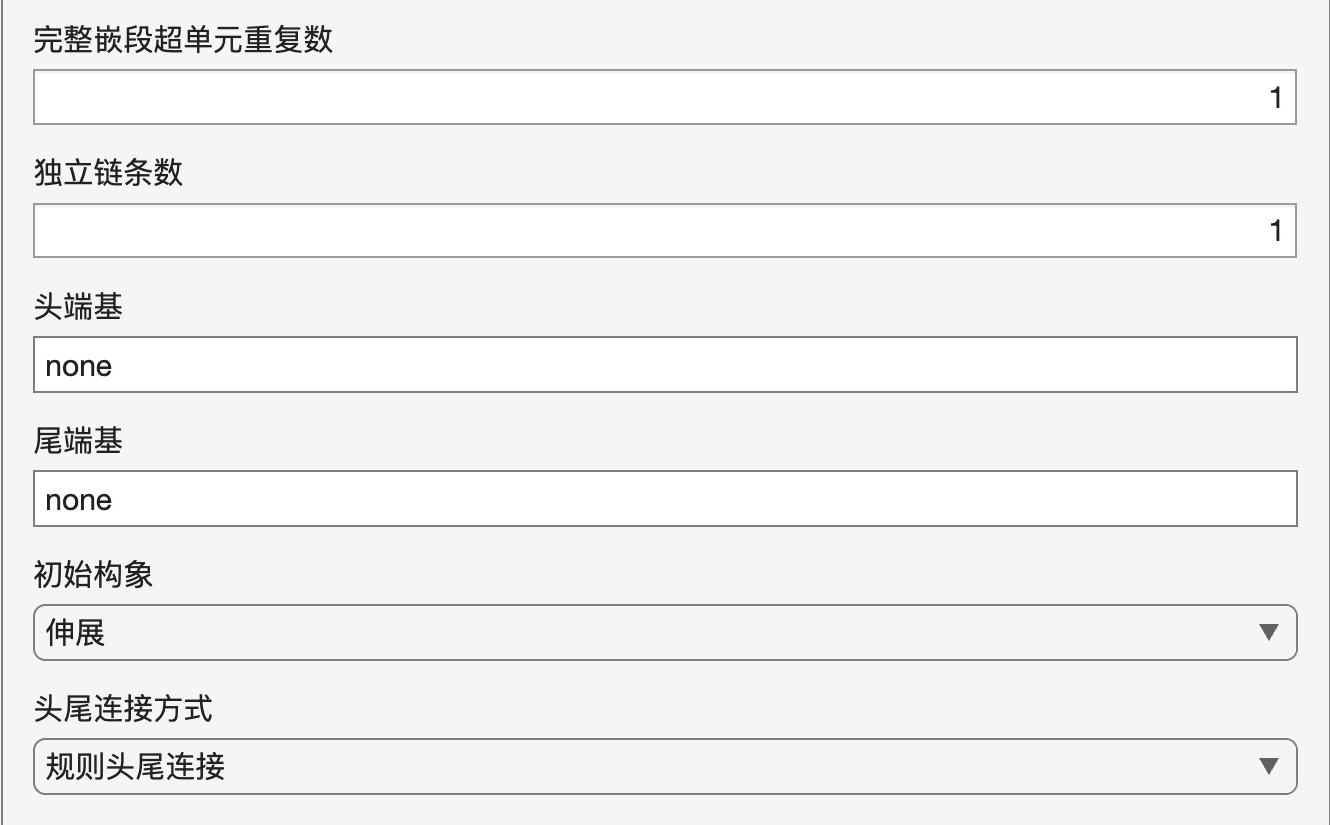
\includegraphics[width=\linewidth]{publication-assets/crop-14436d05d0623e7cdc6f.png}
\caption{构建PEO--PPO--PEO嵌段链的参数。上方输入\literalinput{PEO PPO PEO}、\literalinput{3 4 3}和种子8；下方设为重复1次、1条链、首尾端基均为\file{none}，初始构象为伸展，采用规则头尾连接。}
\label{fig:polymer-block-parameters}
\end{figure}

\begin{figure}[H]
\centering
% 完整链(165,900,2860,1150)，2695×250；122mm约561ppi。
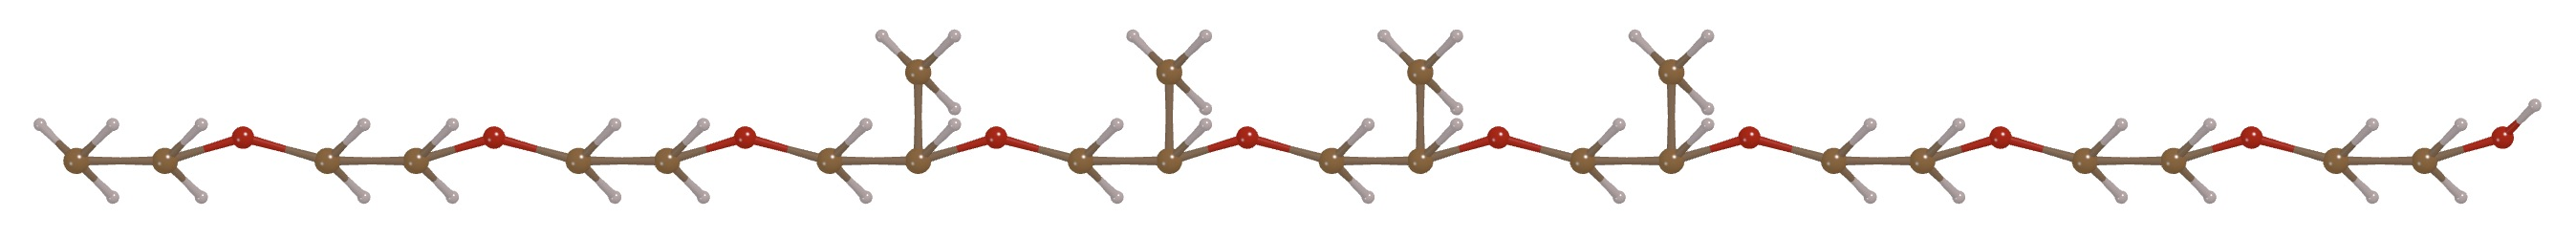
\includegraphics[width=\linewidth]{publication-assets/crop-7684a8a790954b6a1954.png}
\par\vspace{3mm}
\begin{minipage}[t]{40mm}
\vspace{0pt}
% 实际组成摘要(40,330,440,560)，400×230；40mm约254ppi。
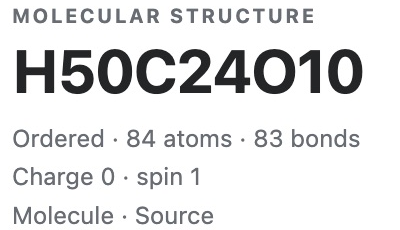
\includegraphics[width=\linewidth]{publication-assets/crop-c77f26280735587ce6a4.png}
\end{minipage}\hfill
\begin{minipage}[t]{80mm}
\vspace{0pt}
% 中部带四个甲基侧支的PPO局部(1000,900,2080,1150)，1080×250；80mm约343ppi。
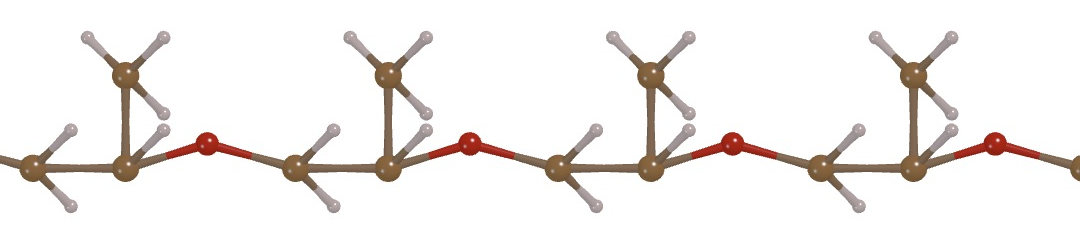
\includegraphics[width=\linewidth]{publication-assets/crop-71a6b6056b817444ef97.png}
\end{minipage}
\caption{应用上述参数后得到的嵌段链初始结构。上方显示整条链；下方左侧摘要为$\mathrm{C_{24}H_{50}O_{10}}$、84个原子和83条连接，右侧放大中部PPO段的四个甲基侧支。}
\label{fig:polymer-block-model}
\end{figure}


\subsection{精確組成的無規鏈}

另建一個分子文件，選擇\ui{構建無規共聚物}，重複單元為 PE、PP，摩爾分數為 0.3、0.7，重複總數為 20，啟用精確組成，種子設為 91。此時組成目標是 6 個 PE 和 14 個 PP 單元；它們在鏈上的具體排列由生成規則和種子確定。

反應性比用於無規序列的終端模型，本例在相應文字框中保持\literalinput{1 1}，初始構象選擇\ui{伸展}，\ui{立構規整性}選擇\ui{間規立構}。生成後應得到 $\mathrm{C_{54}H_{110}}$，共 164 個原子、163 條鍵；隨書\file{PE6-PP14-seed91.json}保留這一結果。它與嵌段鏈的區別首先在於單元排列，而不是檔名或整體輪廓。

\ui{立構規整性}可選擇\ui{間規立構}、\ui{等規立構}或\ui{無規立構}。工具儲存所選立構標記；本組引數在種子不變時，間規與等規選項生成相同座標。本例用於檢查精確組成、序列和連線。研究立構效應時，還需核對側基的實際空間排列。

支鏈高分子以主鏈單元、支鏈片段和連線間隔描述；基礎樹枝狀聚合物以代數、核心官能度和分支因子描述。代數增加會很快擴大原子數量。建立大型結構前先檢視預計規模，先做小模型核對連線，再擴充套件到目標尺寸。

\section{裝填分子混合物}
\index{Hunhewu zhuangtian@混合物裝填}

\subsection{密度與分子數量}

裝填把多個分子放入給定的空間，並滿足最短接觸等幾何條件。它與化學反應或分子動力學平衡不同。目標密度通常以 $\mathrm{g/cm^3}$ 輸入，最短接觸以 \AA 輸入；提高密度會減小可用空間，使裝填更困難。

\ui{構建無定形晶胞}以當前分子為組分，輸入分子數、目標密度、最短接觸和種子。可以先用較少分子完成一次裝填，檢查分子是否完整、晶胞尺寸是否合理，再增加數量。相同分子數並不意味著不同組分具有相同盒子大小，分子質量也參與密度關係。

\ui{裝填混合物}同時使用當前分子與專案中的第二個分子。組成方式可按數量、摩爾分數或質量分數指定。在\ui{組成方式}下拉選單中選擇\ui{精確分子數}，並在\ui{組分分子數}文字框輸入 \literalinput{10 10}，表示兩類分子各 10 個；使用分數模式時，還要給出總分子數。摩爾分數和質量分數對於分子質量不同的組分通常不會產生相同分子個數，應在結果報告中核對實際數量。

\subsection{練習：裝入十個水分子和十個乙醇分子}

匯入\file{water-packing.json}和\file{ethanol-optimized.json}，前者保留水分子的兩條 O--H 連線，後者是第\ref{ch:modeling}章最佳化的乙醇。啟用水分子，開啟\ui{裝填混合物}，在\ui{專案中的第二個分子}下拉選單中選擇乙醇結構。

組成方式選擇\ui{精確分子數}，組分分子數輸入\literalinput{10 10}，目標密度設為 $0.1\,\mathrm{g/cm^3}$，容差為 $1.2\,\text{\AA}$，隨機種子為 23，每批裝填分子數保持 100，密度遞增階段留空。本例採用較疏鬆的初始盒子，便於檢查分子完整性；混合液的平衡密度由後續平衡過程確定。

結果\file{water10-ethanol10-packed.json}含 20 個分子、120 個原子，組成為 $\mathrm{C_{20}H_{80}O_{20}}$。立方盒邊長約為 $21.9954\,\text{\AA}$，按總質量和體積重算的密度為 $0.1\,\mathrm{g/cm^3}$。包括週期映像的最短分子間距離約為 $4.0990\,\text{\AA}$；分子內部距離保持不變。這裡的接觸要求作用於不同分子，不能拿水內部的 O--H 鍵長與它比較。

儲存結果時保留兩份組分輸入。裝填結構記錄了分子和組分編號，輸出不含完整的全域性顯式鍵表；需要繼續處理分子拓撲時，仍要結合原組分的連線資訊。配套指令碼\file{interface_packing_examples.m}提供組分輸入、候選構型和接觸檢查方法。

\subsection{為裝填選擇空間}

\ui{構建受限分子層}增加了限制軸和允許區域，用於將分子集中在盒子中的一部分。輸入前檢視區域按分數還是長度解釋，使上下限與所選軸對應。\ui{裝入已有晶胞}保留當前宿主，把專案分子加入盒子；\ui{繞奈米粒子裝填}還需要宿主周圍的間隔，用於避免直接貼近粒子表面。

裝填失敗時，可以從幾何條件入手：降低初始目標密度或分子數、增大區域、適當調整接觸要求，或更換種子。可選的密度漸增階段和分批裝填用於控制較大任務。完成後檢查分子組成、跨邊界接觸及報告中的未解決問題，再按研究目的進行最小化、熱處理或平衡。

\begin{notebox}{儲存可重複的模型}
對高分子和裝填模型，建議同時保留重複單元或組分、數量與密度、種子、構象、接觸條件，以及生成後的結構。只記錄種子而遺漏其餘引數，不能完整說明模型的來源。將這些資訊與專案一起儲存，之後重建或比較模型會更方便。
\end{notebox}
